% Settings for the default beamer theme
\documentclass[english, aspectratio=169]{beamer}
\usepackage[T1]{fontenc}
\usepackage[utf8]{inputenc}
\usepackage{tabularx}
\usepackage{babel}
\usepackage[ruled,vlined]{algorithm2e}
\SetAlgorithmName{Algoritmus}{algoritmus}{List of Algorithms}
\setcounter{secnumdepth}{3}
\setcounter{tocdepth}{3}

\makeatletter

\newcommand\makebeamertitle{\frame{\maketitle}}

% (ERT) argument for the TOC
\AtBeginDocument{%
  \let\origtableofcontents=\tableofcontents
  \def\tableofcontents{\@ifnextchar[{\origtableofcontents}{\gobbletableofcontents}}
  \def\gobbletableofcontents#1{\origtableofcontents}
}

% Theme settings
\usetheme{Frankfurt}
\usecolortheme{default}
\usefonttheme[onlymath]{serif}

% Template settings
\setbeamertemplate{navigation symbols}{}
\setbeamertemplate{blocks}[rounded][shadow=false]
\setbeamertemplate{title page}[default][colsep=-4bp, rounded=true, shadow=false]
\makeatother

\begin{document}

% Title page
\section{Bevezetés}
\title[]{Üzleti Intelligencia}
\subtitle{10. Előadás: Visszacsatolásos neurális hálózatok}
\author[Kuknyó Dániel]{Kuknyó Dániel\\Budapesti Gazdasági Egyetem}
\date{2023/24\\1.félév}
\makebeamertitle

% Table of contents slide
\begin{frame}
\tableofcontents{}
\end{frame}

% Table of contents of the current section
\begin{frame}
\tableofcontents[currentsection]
\end{frame}


\begin{frame}{Visszacsatolásos neurális hálózatok alapjai}
\renewcommand{\arraystretch}{2.}
\begin{tabularx}{\textwidth}{m{4cm}m{5cm}m{5cm}}
\textbf{Alkalmazás} & \textbf{Input} & \textbf{Output} \\
	Beszédfelismerés & 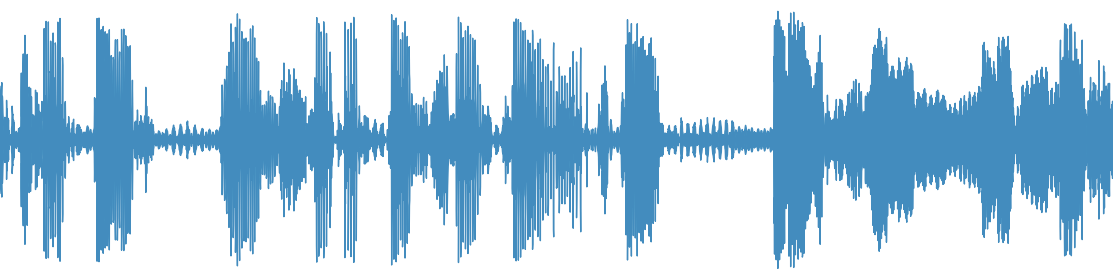
\includegraphics[width=.25\textwidth, keepaspectratio]{images/recurrent_1.png} & "Milyen szép időnk van ma!" \\
	Szemantikai értelmezés & "Ez egy rossz film volt." & 
\includegraphics[width=.2\textwidth, keepaspectratio]{images/recurrent_2.png} \\
	DNS szekvencia elemzés & AGCCCTGTACTAG & AGC\textcolor{red}{CCTGT}ACTAG \\
	Gépi fordítás & "Willst du mit mir tanzen?" & "Szeretnél velem táncolni?" \\
	Videók elemzése & 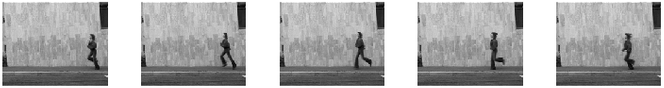
\includegraphics[width=.3\textwidth, keepaspectratio]{images/recurrent_3.png} & Futás \\
	Nevek felismerése & Tegnap Józsi letörölte a\par termelési adatbázist. & Tegnap
\textcolor{red}{Józsi} letörölte a\par termelési adatbázist. \\
\end{tabularx}
\end{frame}

\begin{frame}{Visszacsatolásos hálózatok: nevek felismerése a szövegben}
\renewcommand{\arraystretch}{3.}
\begin{tabularx}{\textwidth}{m{4cm}m{10cm}}
\textbf{Input:} & Tegnap \textcolor{red}{Józsi} letörölte a termelési adatbázist.\\
\textbf{Input reprezentáció:} & $X = \left[ x_{1},\;x_{2},\;x_{3},\;...,\;x_{t},\;...,\;x_{6} \right]$\\
\textbf{Output reprezentáció:} & $Y = \left[ y_{1},\;y_{2},\;y_{3},\;...,\;y_{t},\;...,\;y_{6} \right]$\\
\textbf{Output:} & $\left[ 0,\; \textcolor{red}{1},\; 0,\; 0,\; 0,\; 0\right]$\\
\end{tabularx}
\end{frame}

\begin{frame}{Szavak reprezentálása 1-hot vektorokkal}
\begin{columns}
\begin{column}{.3\textwidth}
\begin{flushright}
\renewcommand{\arraystretch}{2}
\begin{tabular}{|c|}
\hline
\textbf{Osztály}\\
\hline
Macska\\
\hline
Kutya\\
\hline
Teknős\\
\hline
\end{tabular}
\end{flushright}
\end{column}
\begin{column}{.1\textwidth}
\begin{center}
\begin{Huge}
$\longrightarrow$
\end{Huge}
\end{center}
\end{column}
\begin{column}{.6\textwidth}
\begin{flushleft}
\renewcommand{\arraystretch}{2}
\begin{tabular}{|c|c|c|}
\hline
\textbf{Macska} & \textbf{Kutya} & \textbf{Teknős}\\
\hline
$1$ & $0$ & $0$\\
\hline
$0$ & $1$ & $0$\\
\hline
$0$ & $0$ & $1$\\
\hline
\end{tabular}
\end{flushleft}
\end{column}
\end{columns}
\medskip
Az egyes szavak ilyen módon való kódolása lehetővé teszi, hogy egy neurális hálózat felépítse a saját \textbf{szókincsét}, majd különböző szekvenciákat bináris, azonos hosszúságú vektorok halmazaként reprezentáljon.
\end{frame}

\begin{frame}{Miért alkalmatlanok szekvencia feldolgozásra a hagyományos hálózatok?}
\begin{columns}
\begin{column}{.6\textwidth}
\begin{itemize}
	\item A szekvenciák hossza nem előre meghatározott, ezért nem képes változó hosszúságú input adattal dolgozni. 
	\item Nem képes azonos szekvenciák között súlyokat megosztani. 
\end{itemize}
Ezzel szemben az RNN hálózatok:
\begin{itemize}
	\item Változó hosszúságú sorozatokkal működnek.
	\item Hosszútávú függőségeket is meg tudnak tanulni.
	\item Megőrzi az input vektor rendezettségét.
	\item Képes paramétereket megosztani sorozatok között.
\end{itemize}
\end{column}
\begin{column}{.5\textwidth}
\begin{center}
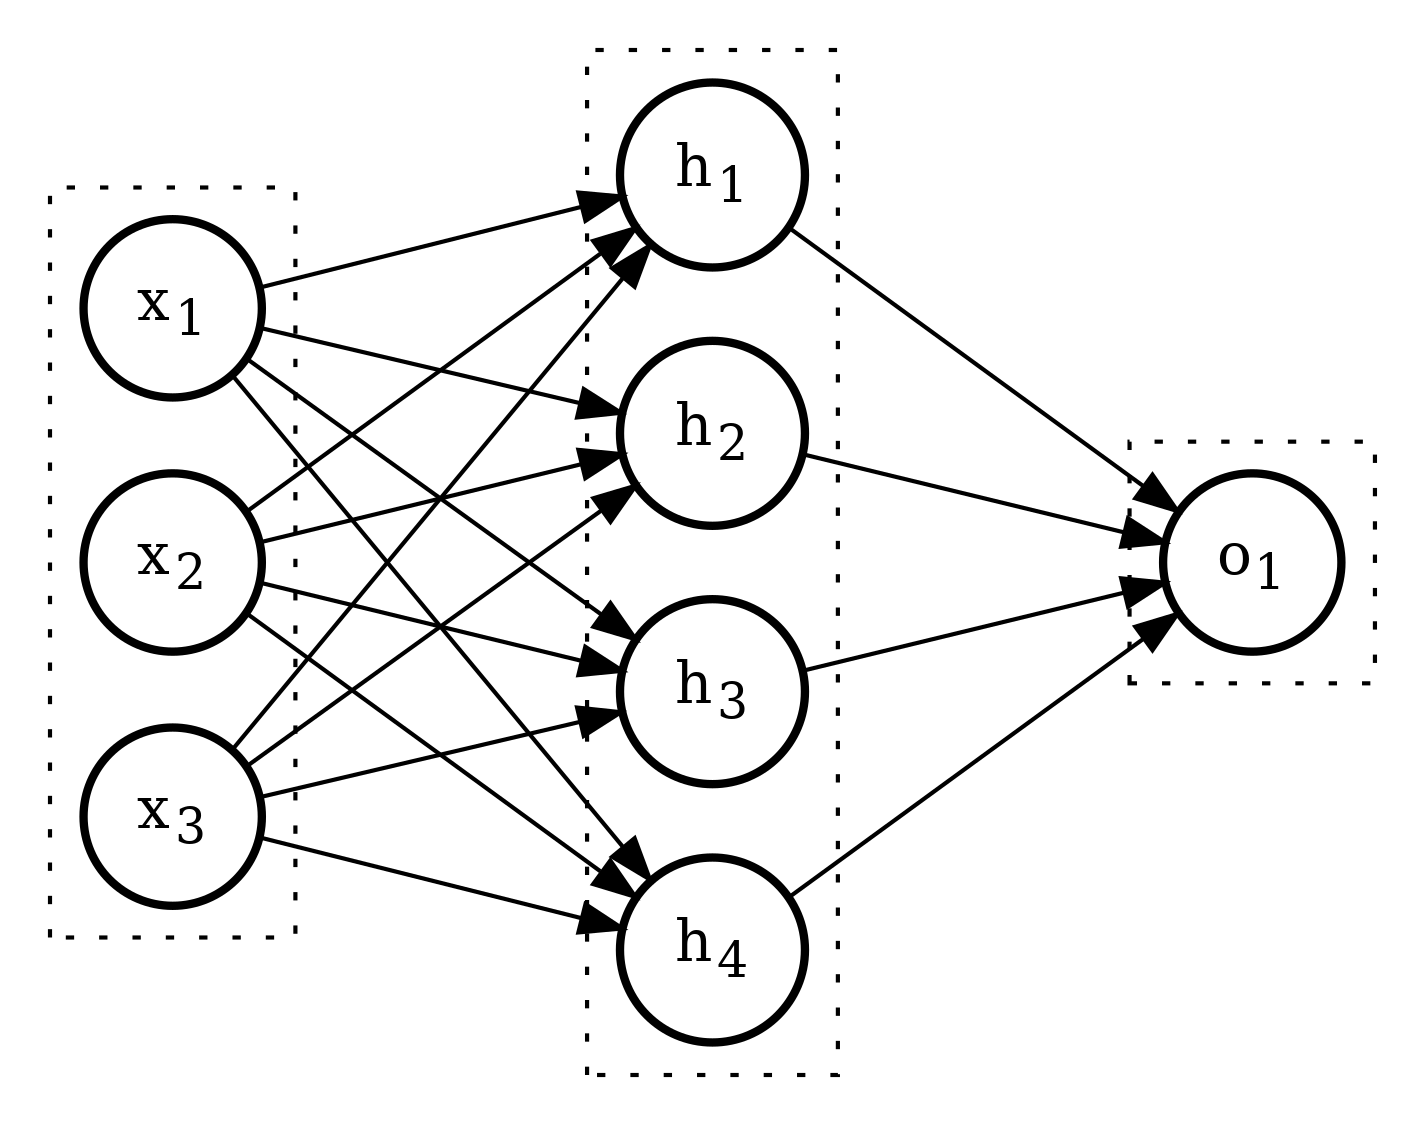
\includegraphics[height=7cm, width=7cm, keepaspectratio]{../../7_dl/doc/graphs/dl_2.png}
\end{center}
\end{column}
\end{columns}
\end{frame}

\section{Visszacsatolásos hálózatok}

\begin{frame}
\tableofcontents[currentsection]
\end{frame}

\begin{frame}{Mélyhálózatok (DNN) vs. visszacsatolásos hálózatok (RNN)}
\begin{columns}
\begin{column}{.3\textwidth}
\begin{center}
Hagyományos mélyhálózat
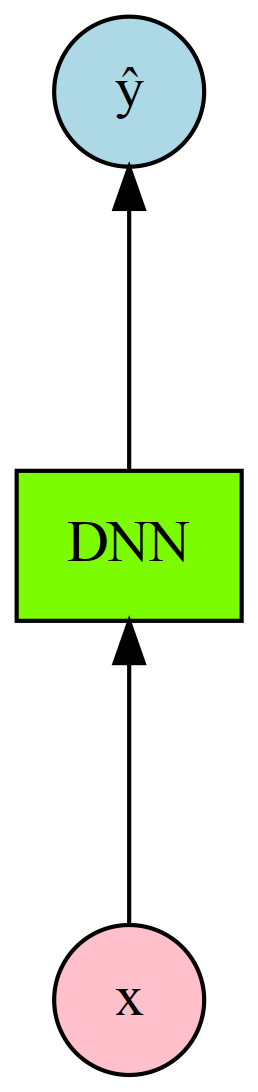
\includegraphics[height=6cm, keepaspectratio]{graphs/recurrent_1.png}
\end{center}
\end{column}
\begin{column}{.3\textwidth}
\begin{center}
Visszacsatolásos mélyhálózat működése
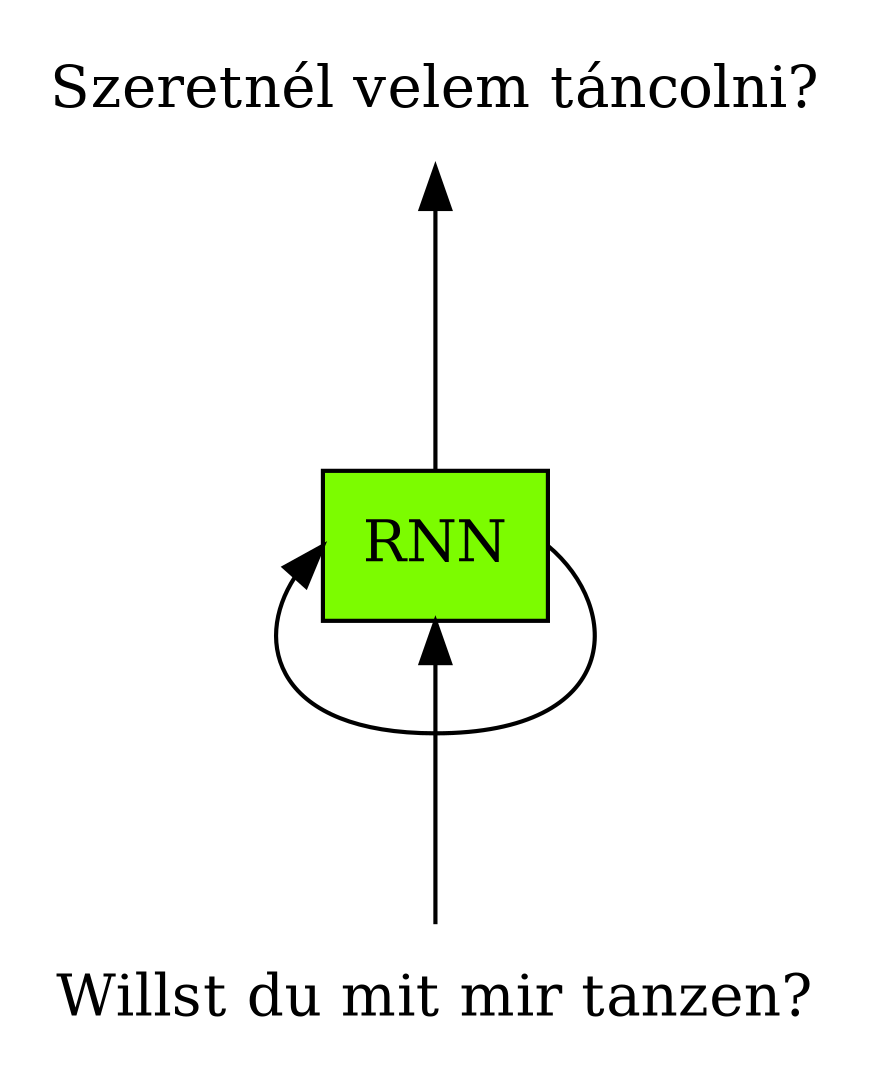
\includegraphics[height=6cm, keepaspectratio]{graphs/recurrent_2.png}
\end{center}
\end{column}
\begin{column}{.3\textwidth}
\begin{center}
Visszacsatolásos mélyhálózat jelölése
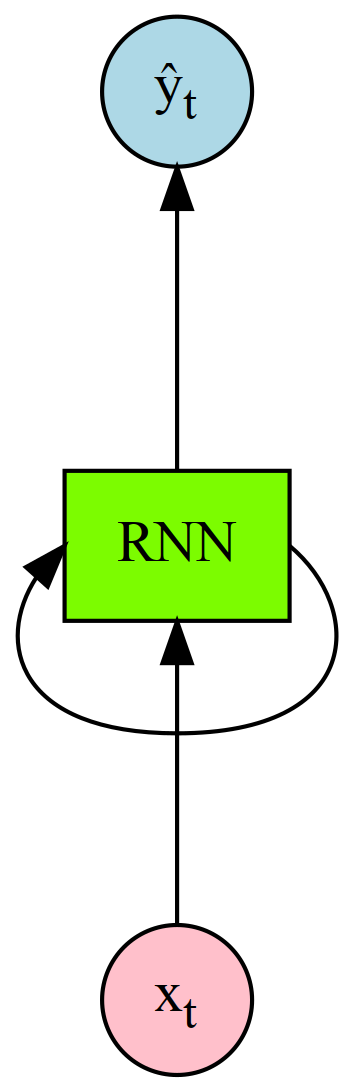
\includegraphics[height=6cm, keepaspectratio]{graphs/recurrent_3.png}
\end{center}
\end{column}
\end{columns}
\end{frame}

\begin{frame}{Reprezentáció}
A visszacsatolásos neurális hálókat kétféle módon lehet jelölni: összehajtott és lehajtott állapotban. Az összehajtott jóval kompaktabb, a lehajtott viszont egy tiszta és intuitív nézőpontot ad a hálózat architektúrájára.
\begin{columns}
\begin{column}{.2\textwidth}
\begin{center}
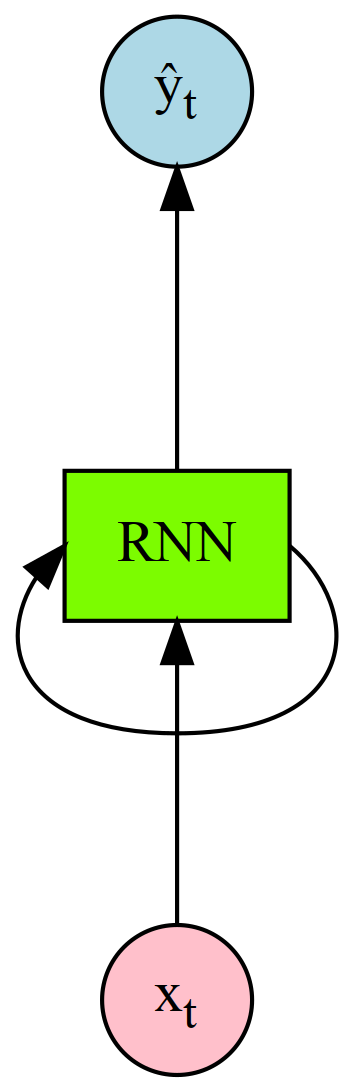
\includegraphics[height=5.5cm, width=\textwidth, keepaspectratio]{graphs/recurrent_3.png}
\end{center}
\end{column}
\begin{column}{.1\textwidth}
\begin{center}
\begin{Huge}
$=$
\end{Huge}
\end{center}
\end{column}
\begin{column}{.7\textwidth}
\begin{center}
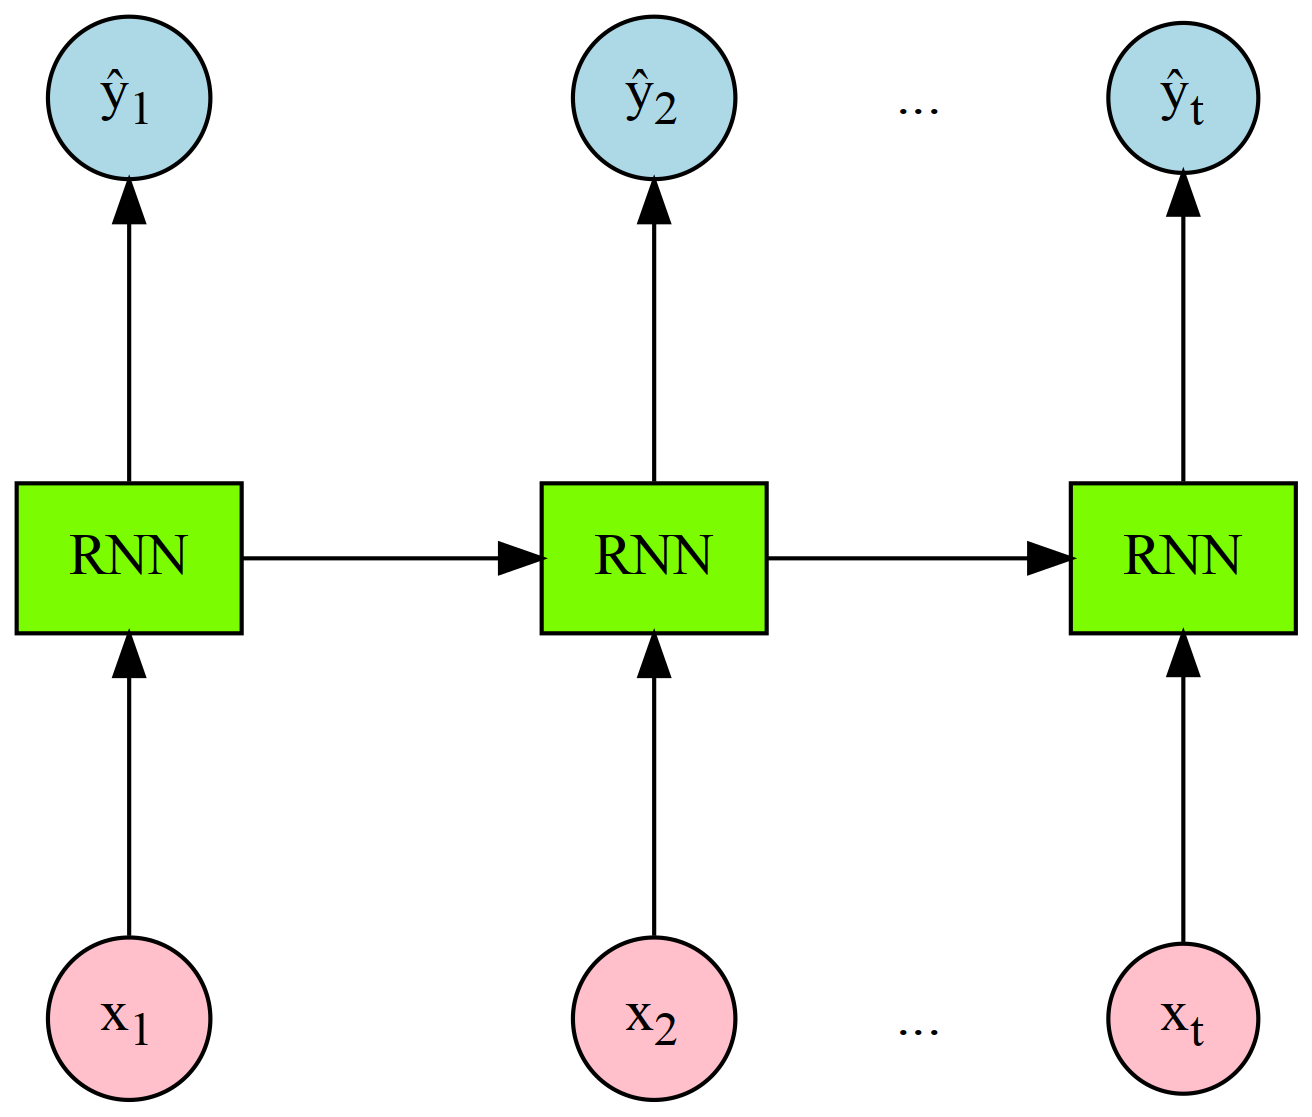
\includegraphics[height=5.5cm, width=\textwidth, keepaspectratio]{graphs/recurrent_4.png}
\end{center}
\end{column}
\end{columns}
\end{frame}

\begin{frame}{Súlyok és kapcsolatok}
\begin{columns}
\begin{column}{.4\textwidth}
\hspace{-2cm}
\begin{itemize}
	\item $x_t$: Input vektor $t$. eleme.
	\item $\hat{y}_t$: Output vektor $t$. eleme.
	\item $h_t$: Rejtett réteg aktivációja (\textbf{cella állapota}) $t$ időben.
	\item $W_x$: Input súlyai \\(időben állandó, tanítható).
	\item $W_y$: Output súlyai \\(időben állandó, tanítható).
\end{itemize}
Ebben az esetben az output
\begin{block}{}
\vspace{-0.2cm}
\[
\hat{y}_t = f(x_t, h_{t-1})
\]
\end{block}
$x_t$ aktuális input és $h_{t-1}$ előző állapot függvénye.
\end{column}
\begin{column}{.7\textwidth}
\begin{center}
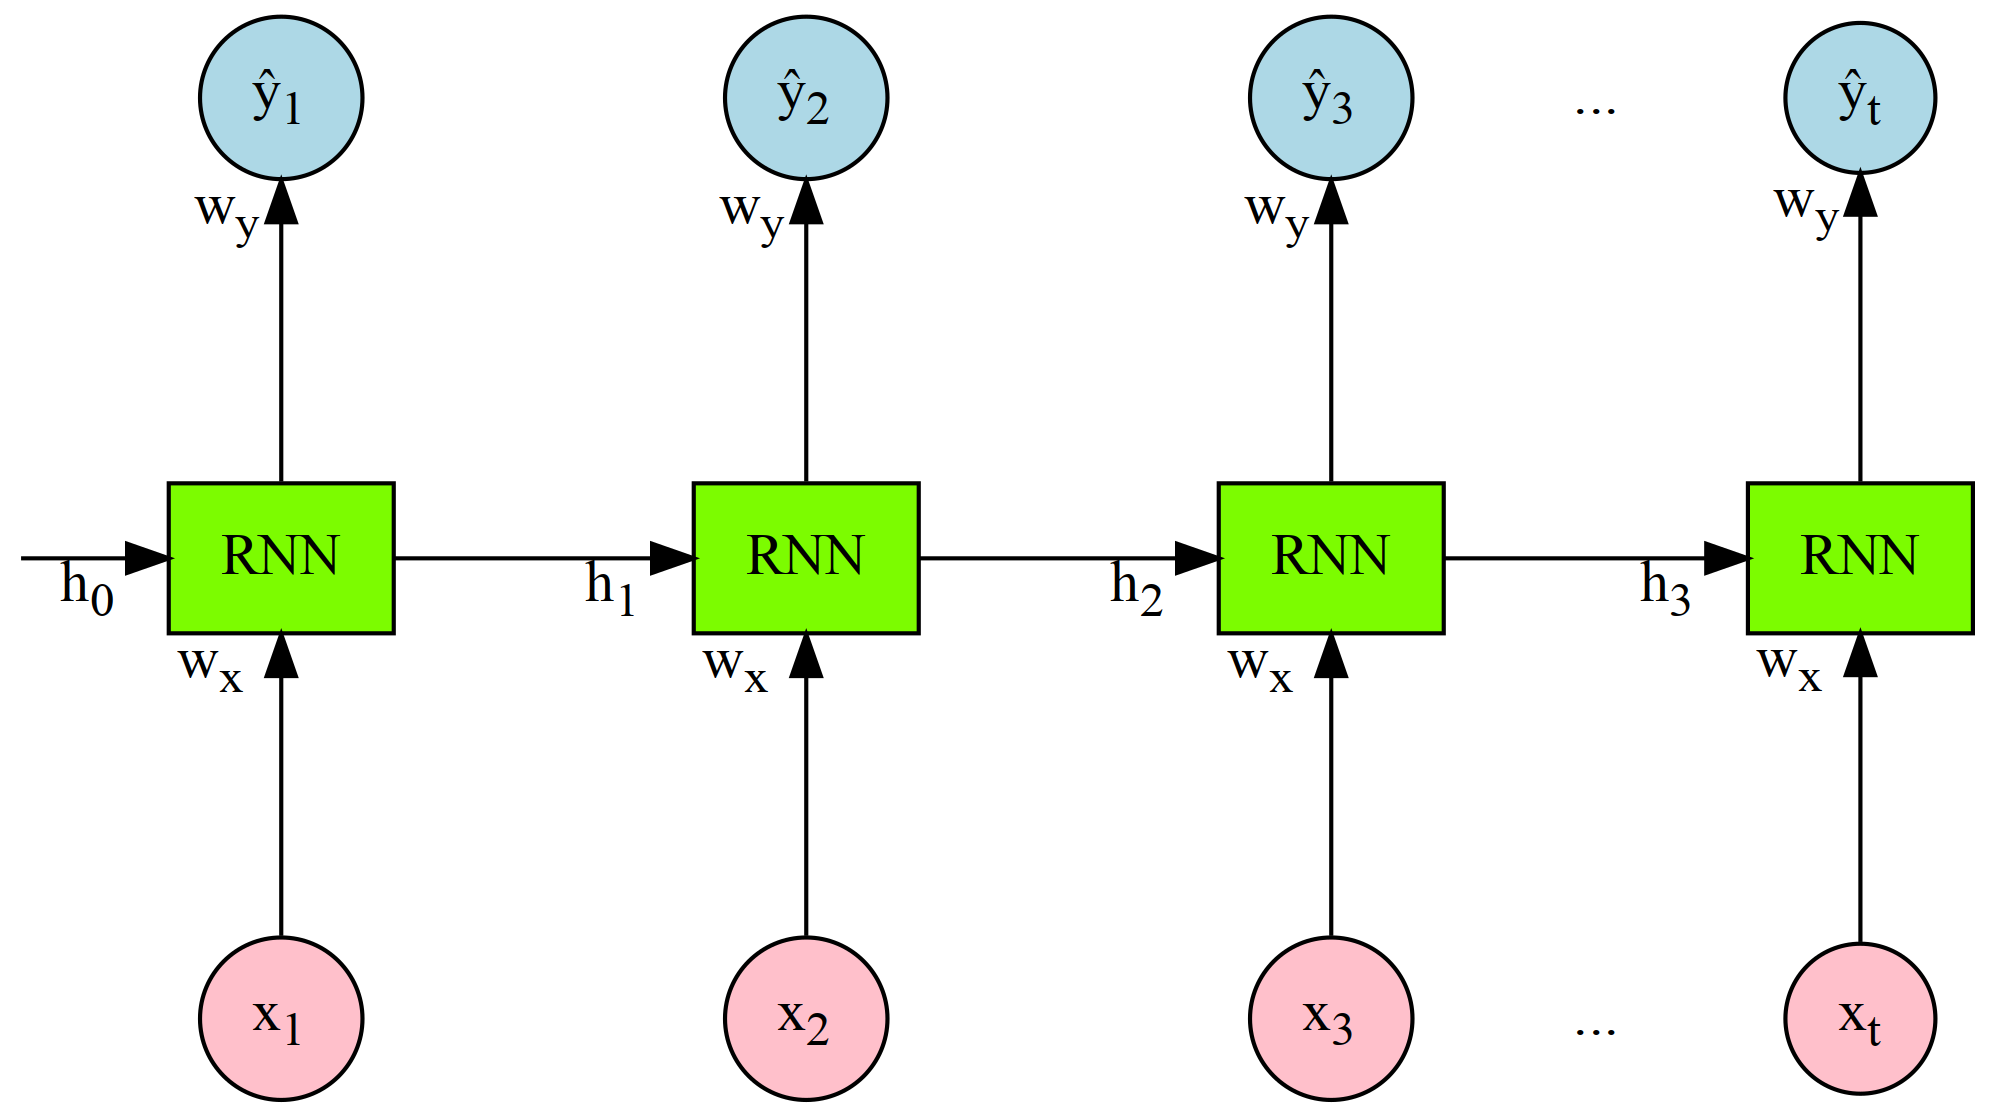
\includegraphics[width=9.5cm, keepaspectratio]{graphs/recurrent_5.png}
\end{center}
\end{column}
\end{columns}
\end{frame}

\begin{frame}{Számítások az RNN-ben}
\begin{columns}
\begin{column}{.5\textwidth}
\begin{block}{Rejtett állapot számítása}
\[
h_t = tanh\left(W_h \cdot h_{t-1} + W_x \cdot x_t + b_h\right)
\]
Ahol $tanh(\cdot)$ a hiperbolikus tangens függvény, $h_{t-1}$ az előző cella állapota, $x_t$ az input vektor aktuális eleme, $b$ pedig a cella torzítása.
\end{block}
\begin{block}{Output számítása}
\[
\hat{y} = tanh\left(W_y \cdot h_t + b_y\right)
\]
\end{block}
\end{column}
\begin{column}{.5\textwidth}
\begin{center}
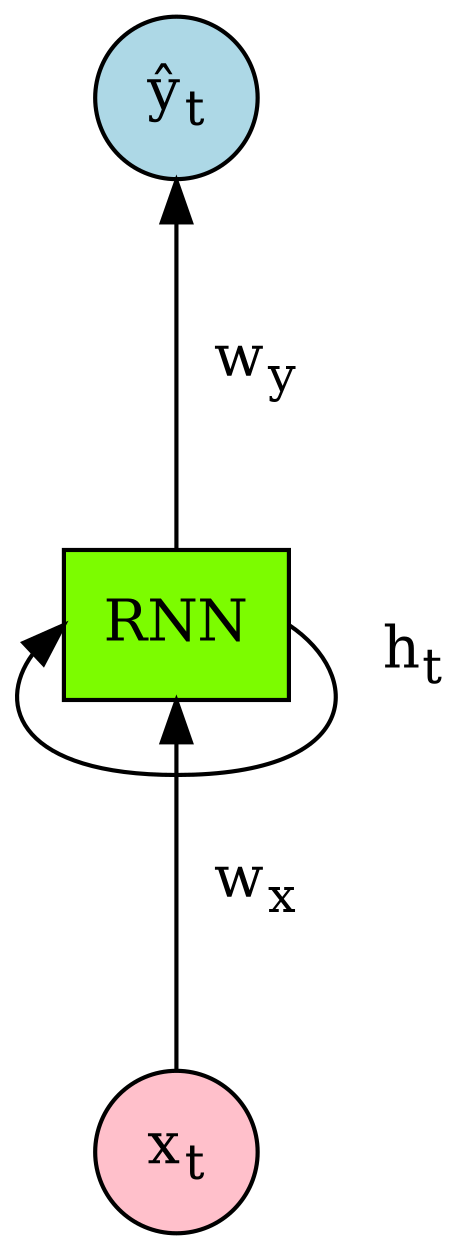
\includegraphics[height=7cm, keepaspectratio]{graphs/recurrent_8.png}
\end{center}
\end{column}
\end{columns}
\end{frame}

\begin{frame}{A hiperbolikus tangens függvény}
\begin{columns}
\begin{column}{.5\textwidth}
A hiperbolikus tangens függvény az egyik gyakori aktivációs függvény visszacsatolásos neurális hálózatokban. Előnyei a \textbf{nemlinearitás}, \textbf{erős gradiens}, \textbf{nulla középpontúság}. 
\begin{block}{Hiperbolikus tangens függvény}
\[
tanh(x) = \frac{e^x - e^{-x}}{e^x + e^{-x}}
\]
Ahol $e \approx 2.71828$ a természetes logaritmus értéke. 
\end{block}
\end{column}
\begin{column}{.5\textwidth}
\begin{center}
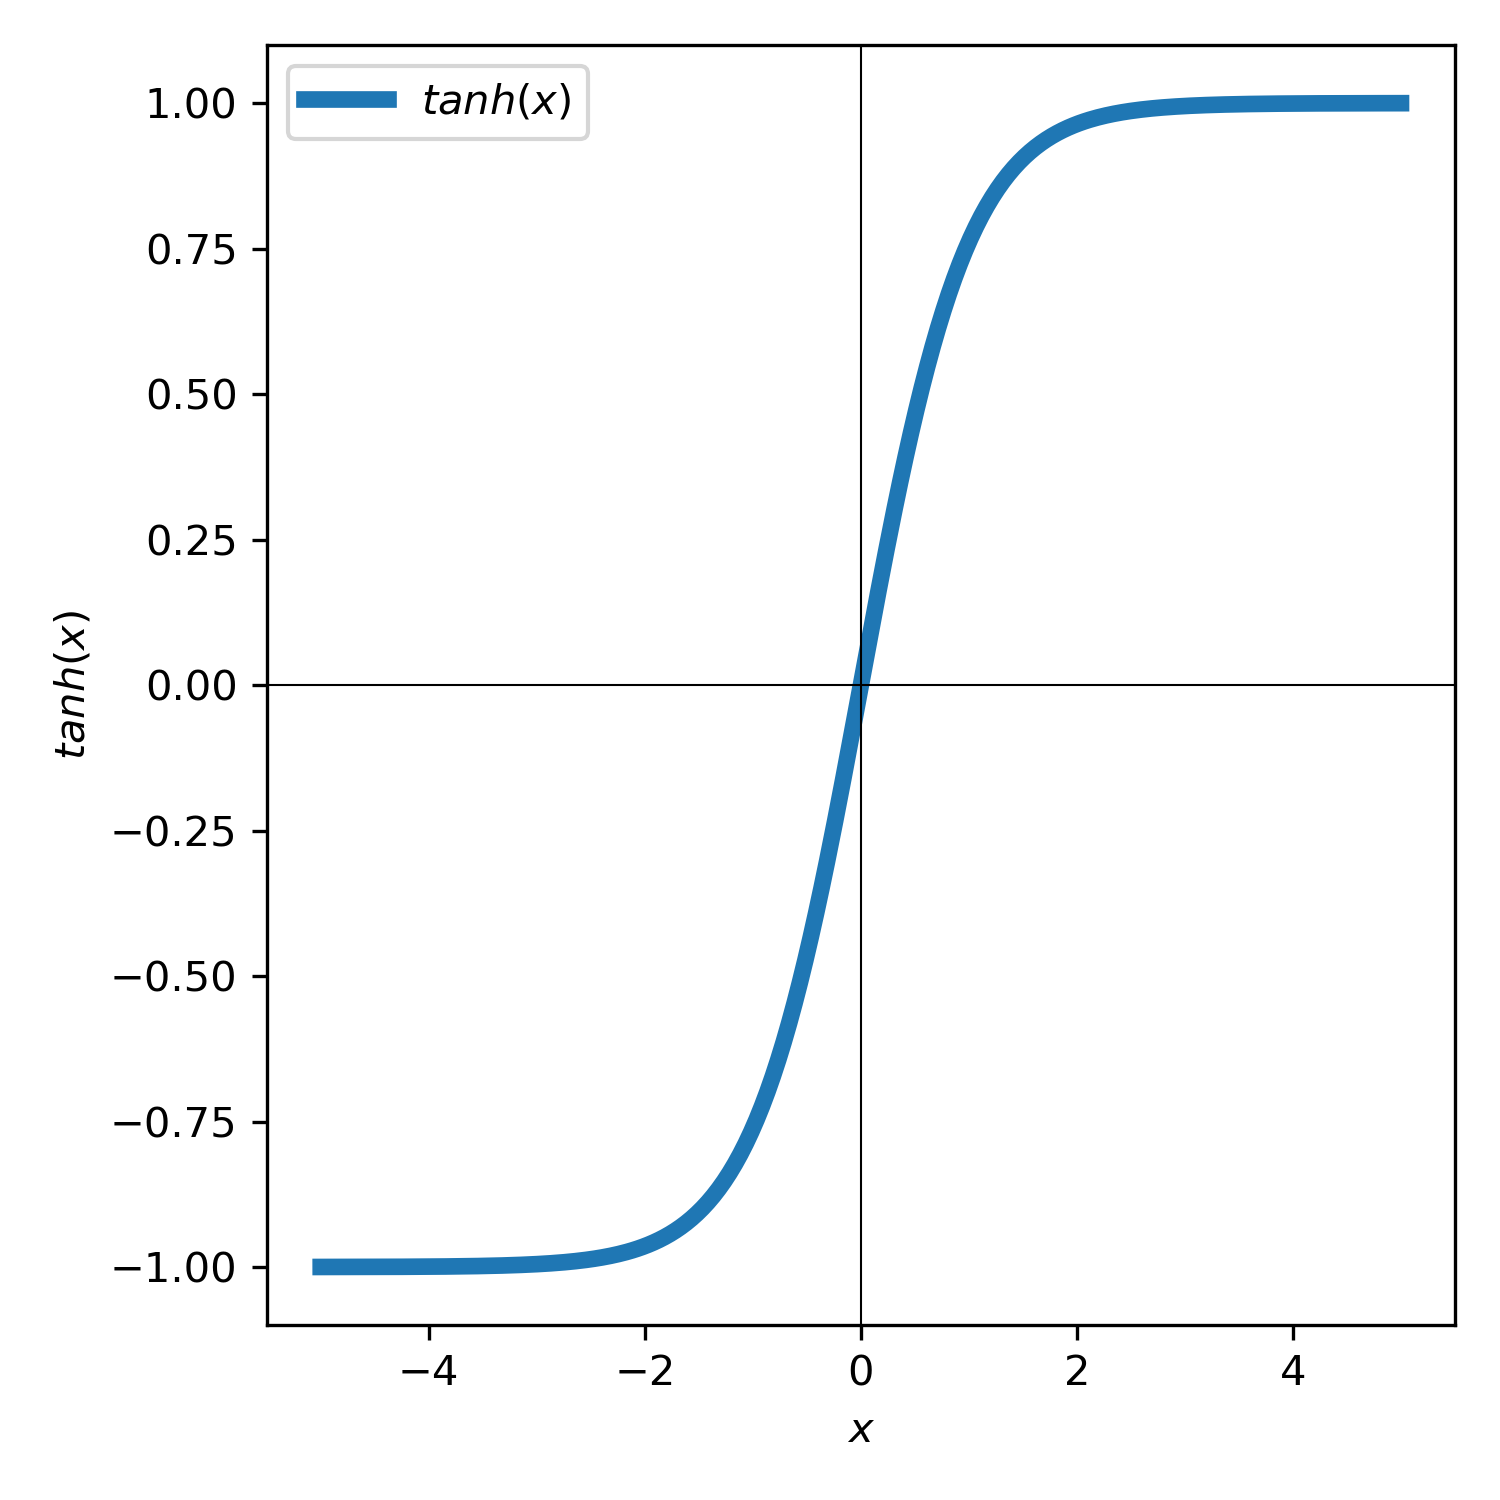
\includegraphics[height=7cm, width=7cm, keepaspectratio]{images/tanh.png}
\end{center}
\end{column}
\end{columns}
\end{frame}

\begin{frame}{Hiba visszaáramoltatás hagyományos hálózatok esetén}
\begin{columns}
\begin{column}{.4\textwidth}
\begin{enumerate}
	\item Köteg előre áramoltatása a hálózaton.
	\item Költség kiszámítása.
	\item Költség gradiensének meghatározása minden paraméter szerint. 
	\item Paraméterek frissítése a költség minimalizálása érdekében.
\end{enumerate}
\end{column}
\begin{column}{.7\textwidth}
\begin{center}
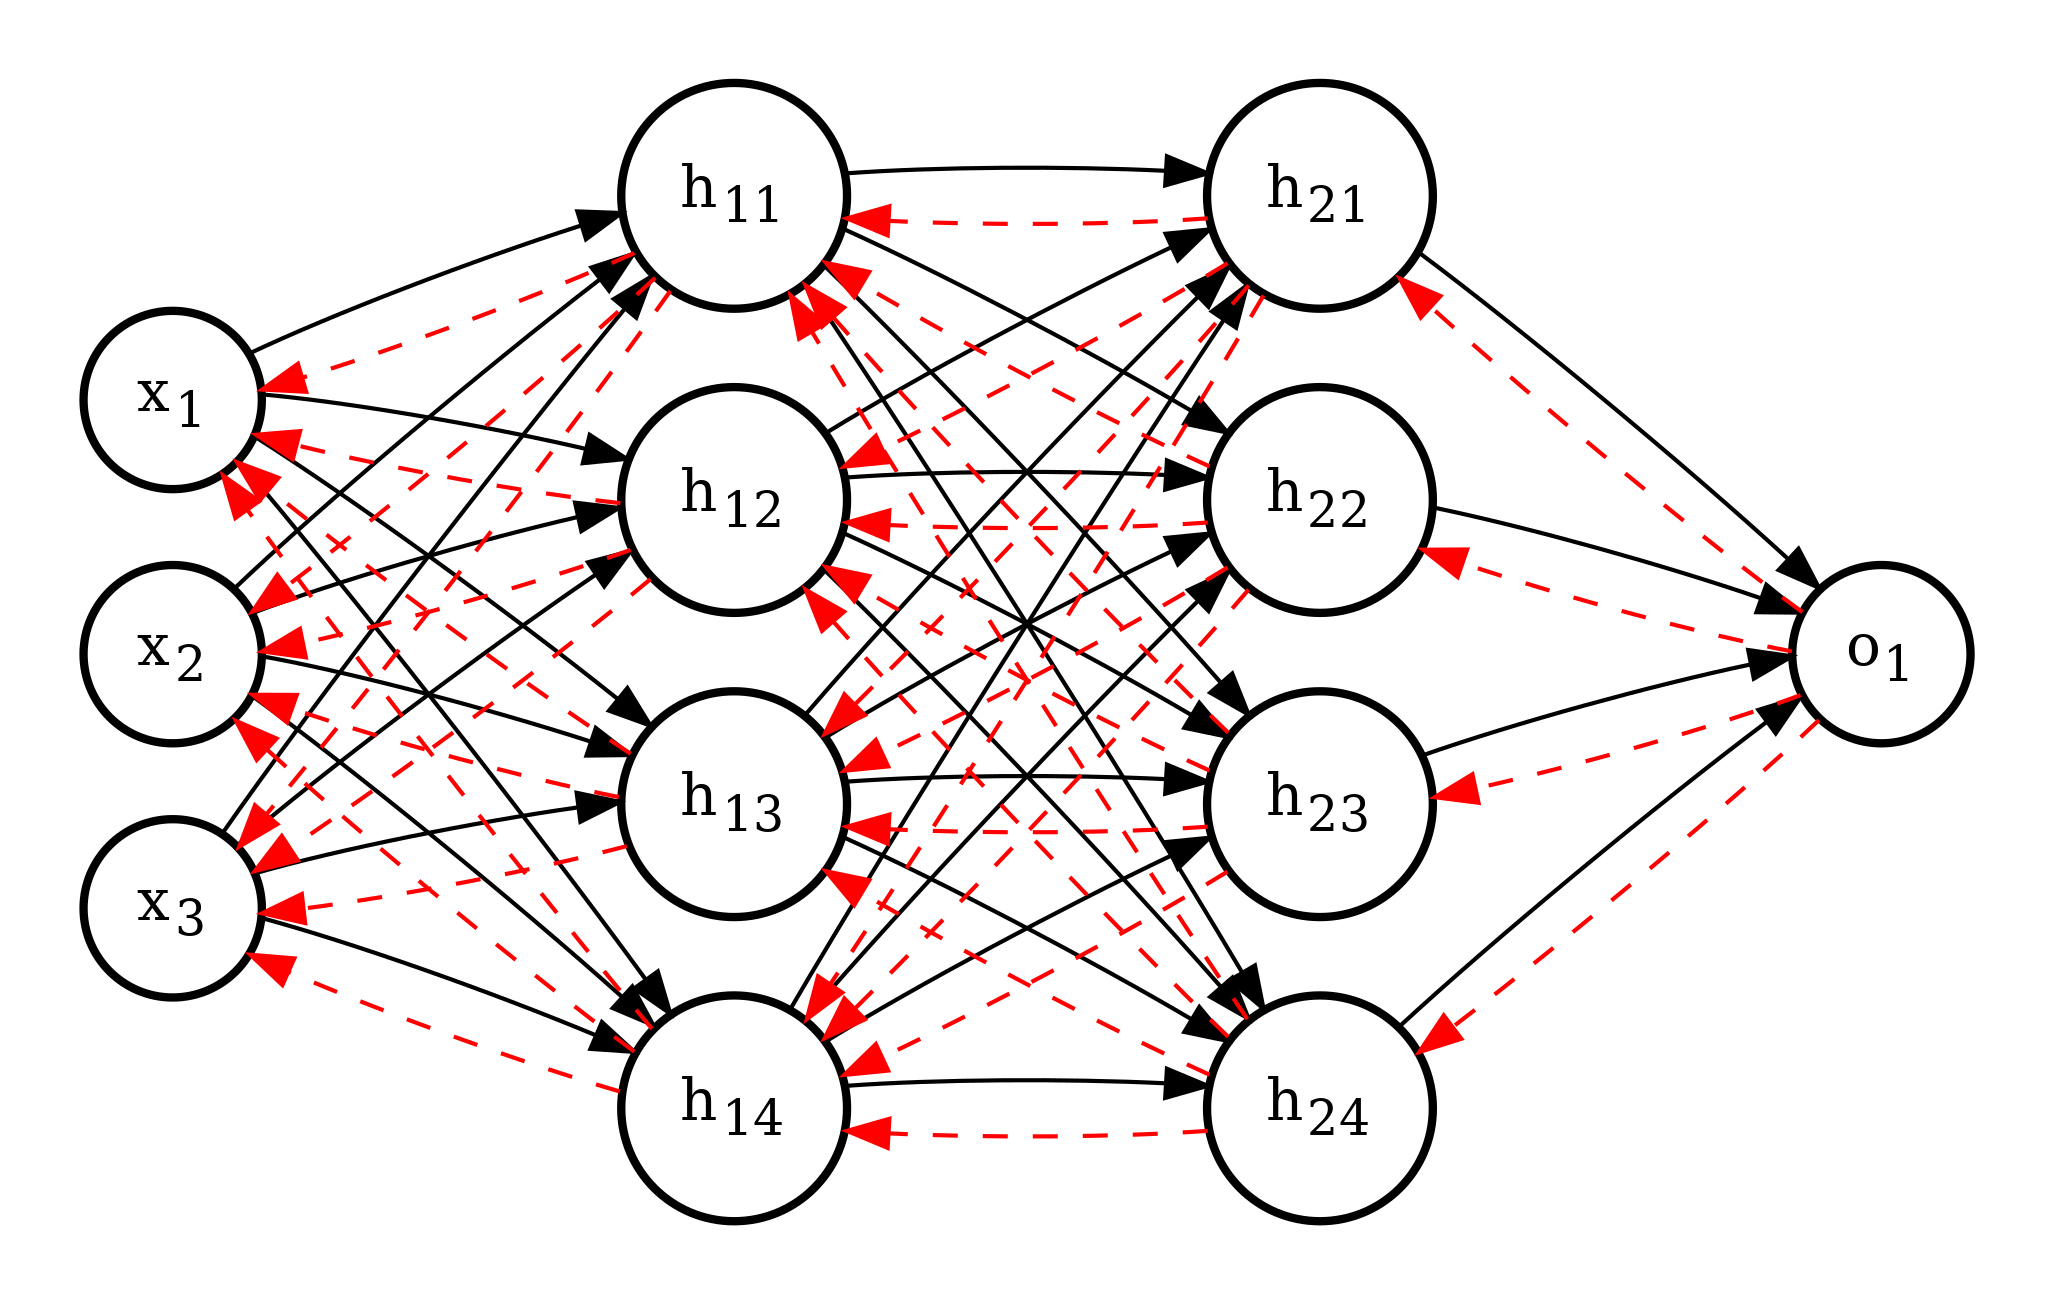
\includegraphics[height=7cm, width=10cm, keepaspectratio]{graphs/recurrent_9.png}
\end{center}
\end{column}
\end{columns}
\end{frame}

\begin{frame}{Hiba kiszámítása RNN esetén: előre áramoltatás}
\begin{columns}
\begin{column}{.5\textwidth}
Előre áramoltatás során az RNN az input szekvencia elemeit \textbf{egyesével dolgozza fel időlépésenként}. \par\smallskip
Minden $t$ időlépésben kiszámolja $L_t$ költséget, amelyet a végén aggregál valamilyen módszerrel, például \textbf{átlagolással vagy összegzéssel}.  
\end{column}
\begin{column}{.5\textwidth}
\begin{center}
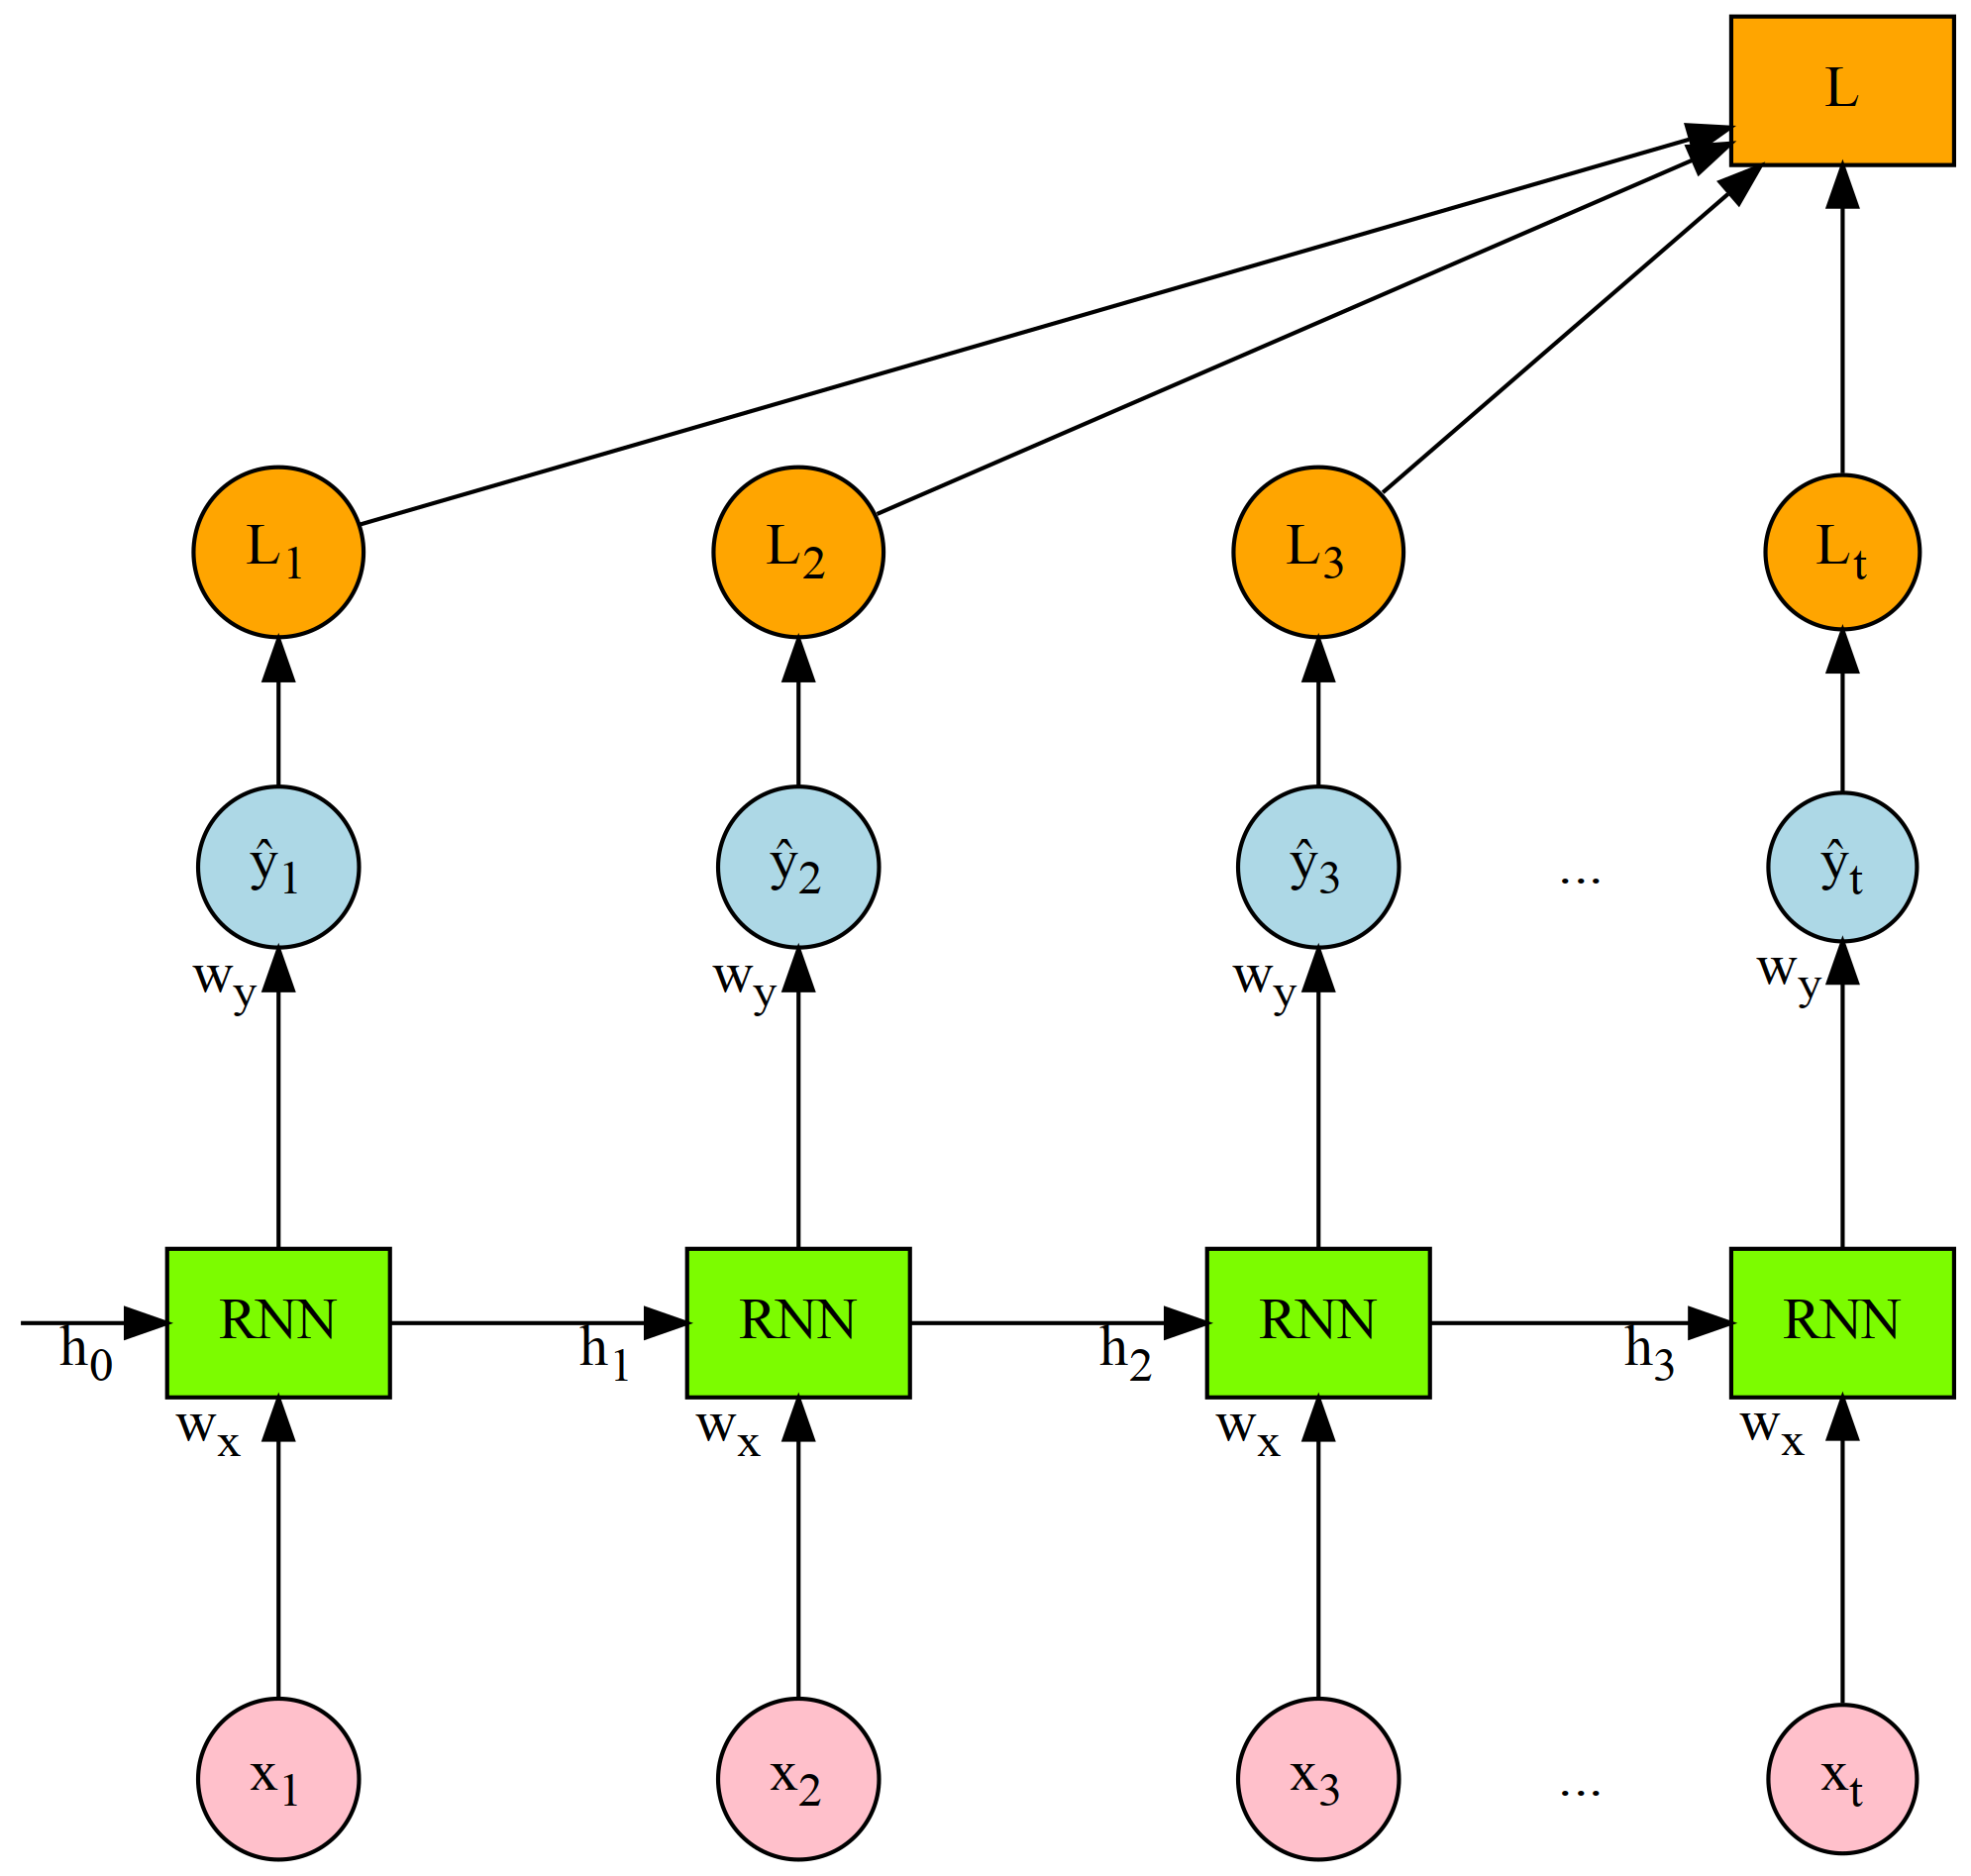
\includegraphics[height=7cm, width=7cm, keepaspectratio]{graphs/recurrent_10.png}
\end{center}
\end{column}
\end{columns}
\end{frame}

\begin{frame}{Hiba kiszámítása RNN esetén: időbeni visszaáramoltatás}
\begin{columns}
\begin{column}{.5\textwidth}
\begin{enumerate}
	\item Az output értékek kiszámítása minden időlépésre. 
	\item A hálózatot lehajtva minden időlépésre a költség kiszámítása.
	\item A hálózatot feltekerve frissíteni a paramétereket. 
	\item Ismétlés a meghatározott lépésszámig.
\end{enumerate}
\end{column}
\begin{column}{.5\textwidth}
\begin{center}
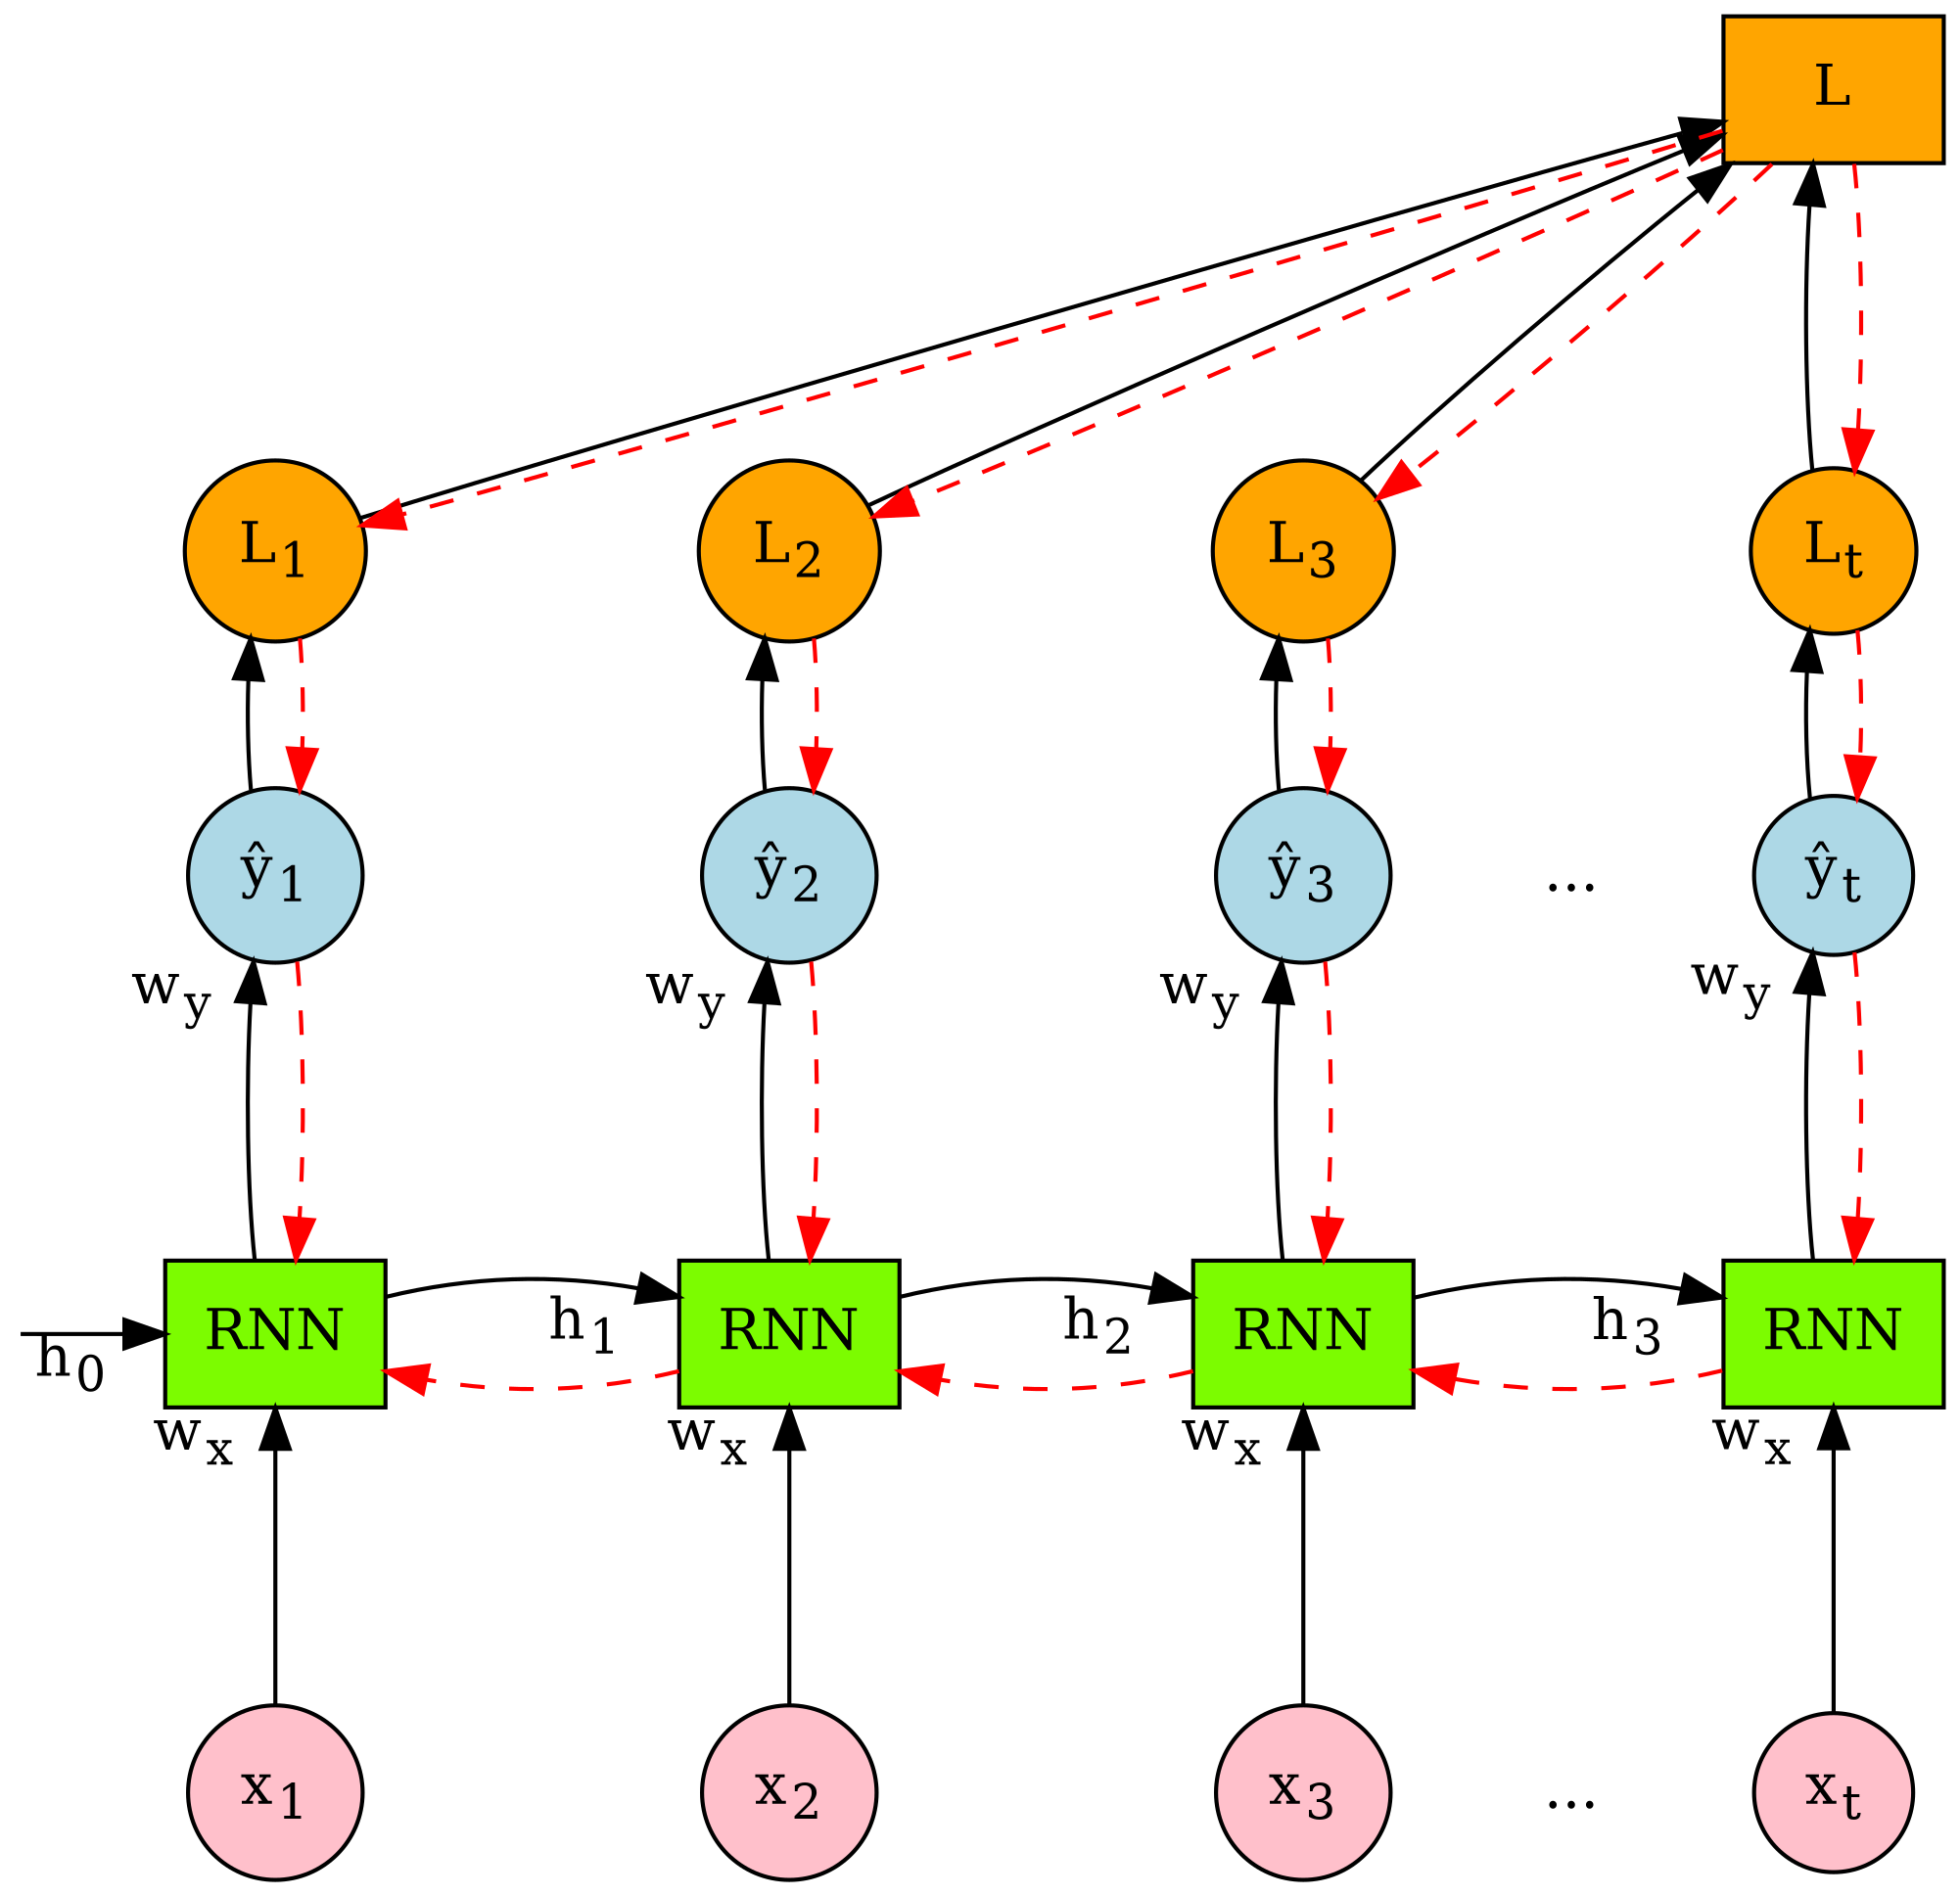
\includegraphics[height=7cm, width=7cm, keepaspectratio]{graphs/recurrent_11.png}
\end{center}
\end{column}
\end{columns}
\end{frame}

\begin{frame}{RNN típusok}
\only<1>{
\begin{center}
\textbf{Egy az egyhez}\par\smallskip
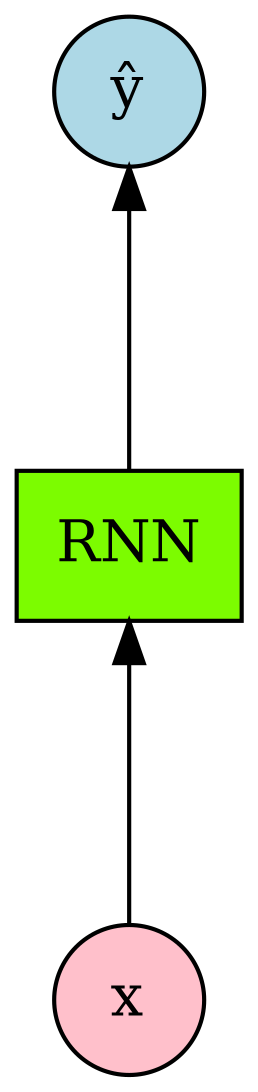
\includegraphics[height=6cm, keepaspectratio]{graphs/recurrent_12.png}
\end{center}}
\only<2>{
\begin{center}
\textbf{Egy az többhöz}\par\smallskip
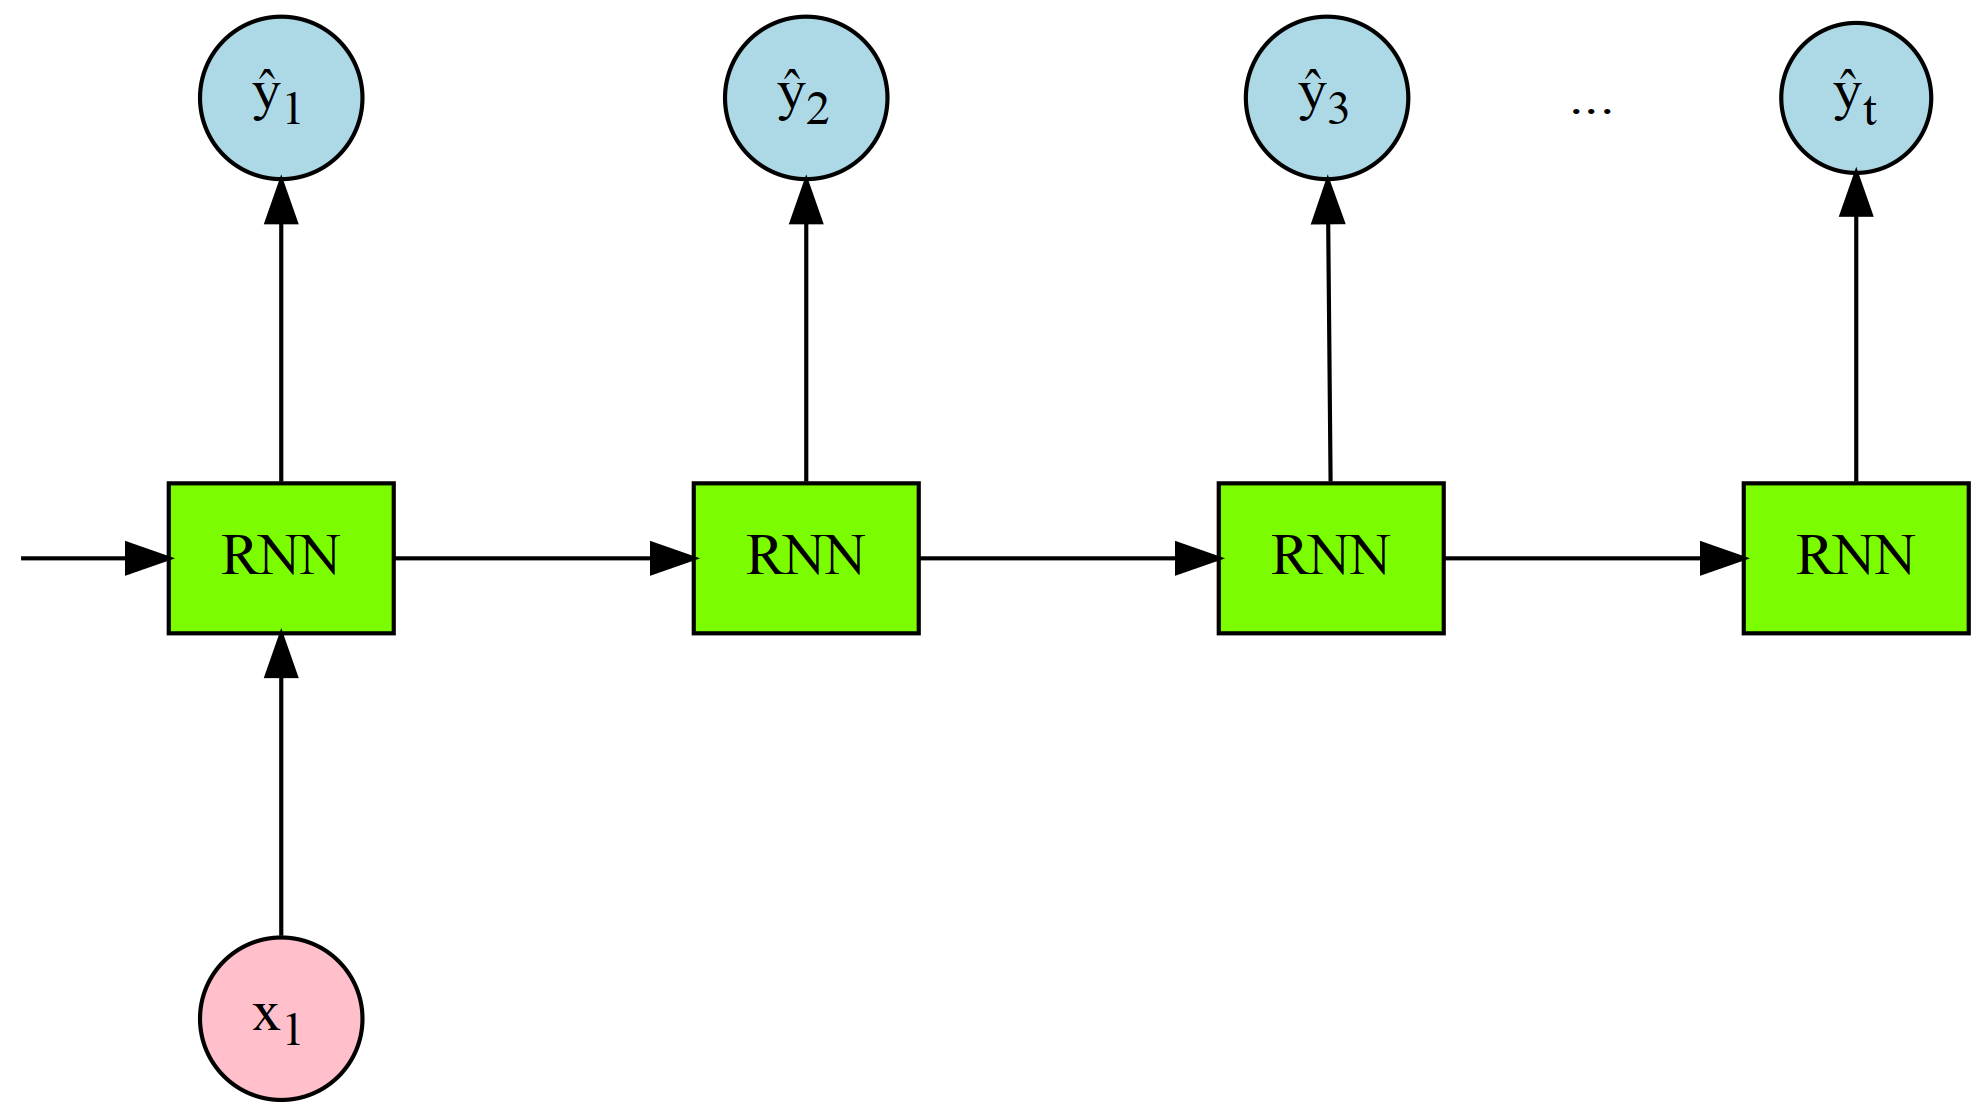
\includegraphics[height=6cm, keepaspectratio]{graphs/recurrent_13.png}
\end{center}}
\only<3>{
\begin{center}
\textbf{Több az egyhez}\par\smallskip
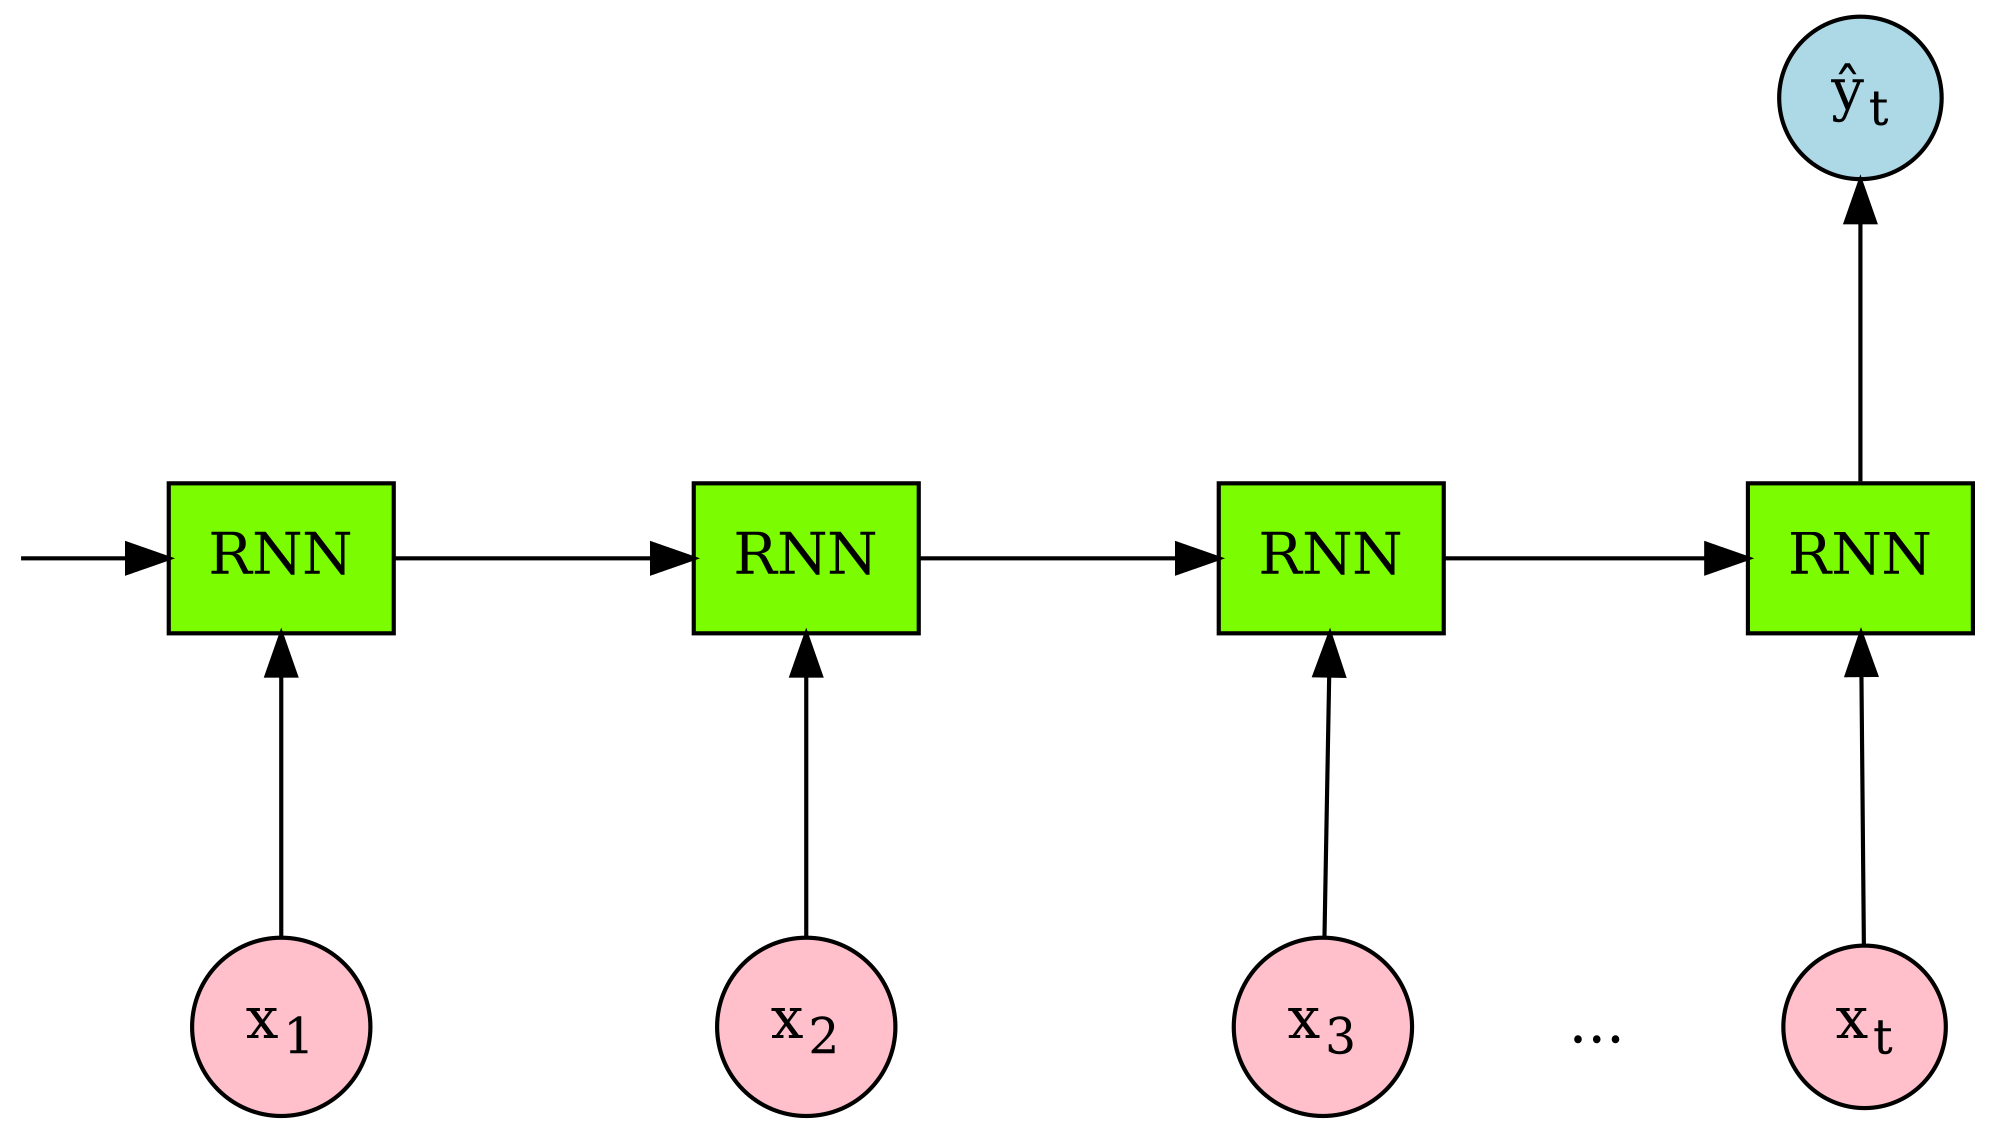
\includegraphics[height=6cm, keepaspectratio]{graphs/recurrent_14.png}
\end{center}}
\only<4>{
\begin{center}
\textbf{Több a többhöz}\par\smallskip
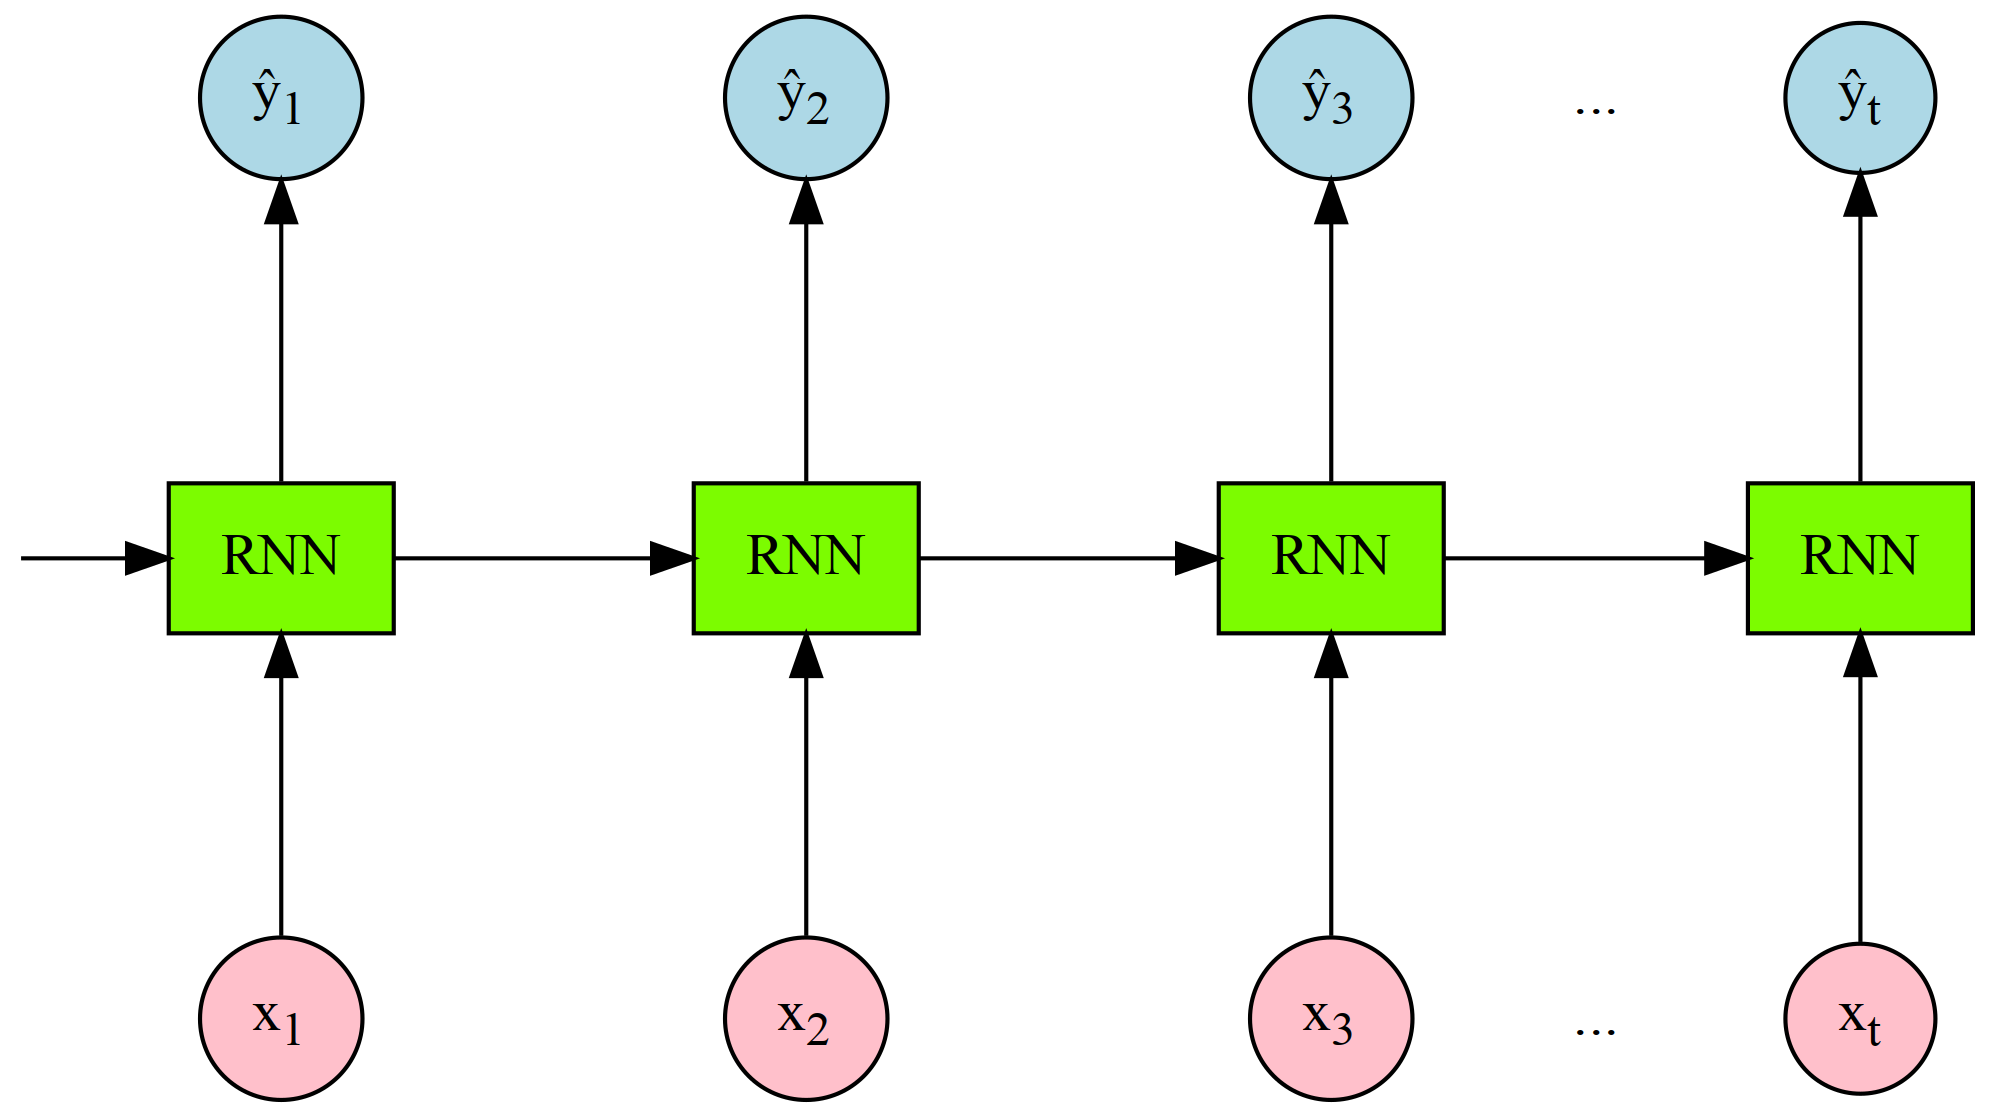
\includegraphics[height=6cm, keepaspectratio]{graphs/recurrent_15.png}
\end{center}}
\only<5>{
\begin{center}
\textbf{Több a többhöz}\par\smallskip
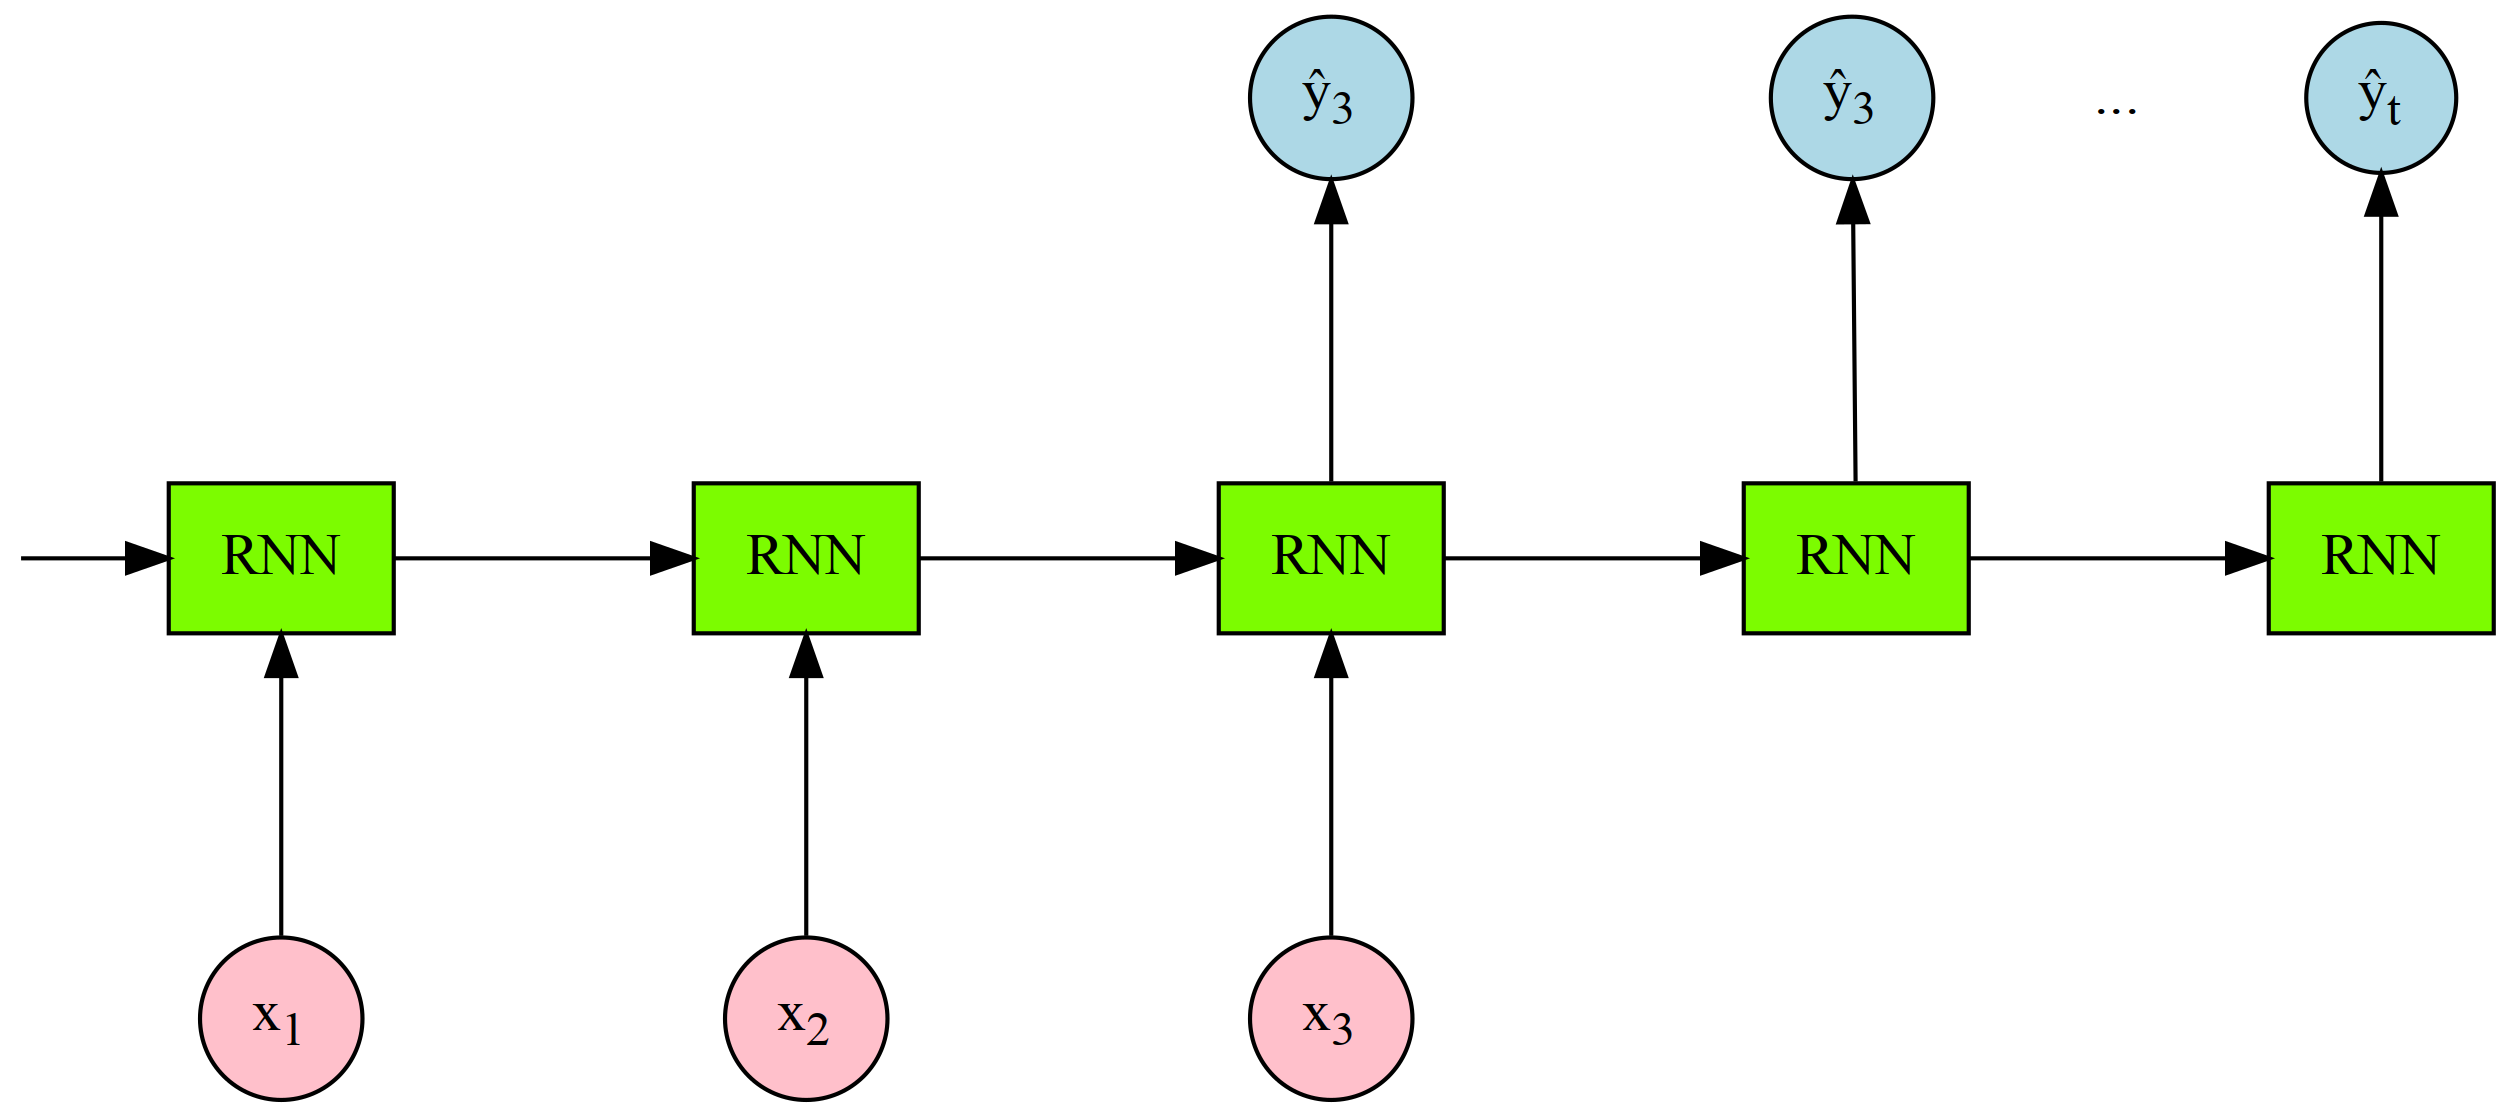
\includegraphics[height=6cm, keepaspectratio]{graphs/recurrent_16.png}
\end{center}}
\only<6>{
\begin{center}
\textbf{Output szerint becsatolt}\par\smallskip
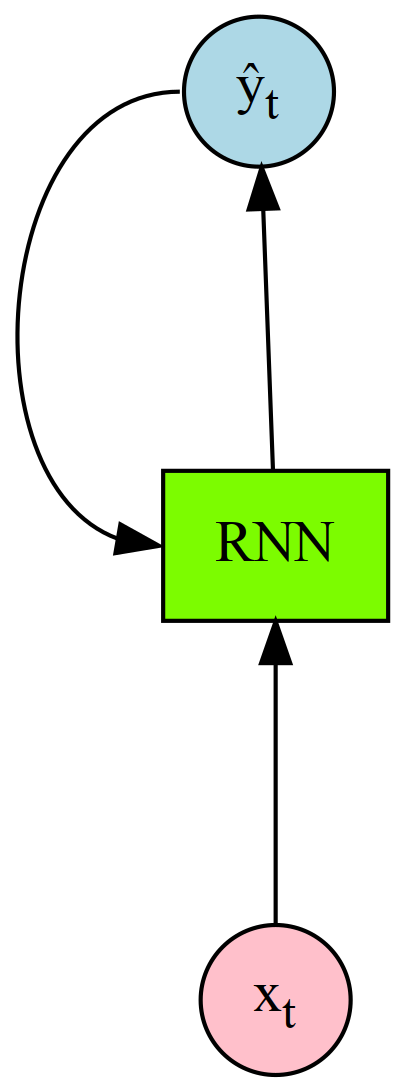
\includegraphics[height=6cm, width=7cm, keepaspectratio]{graphs/recurrent_6.png}
\hspace{2cm}
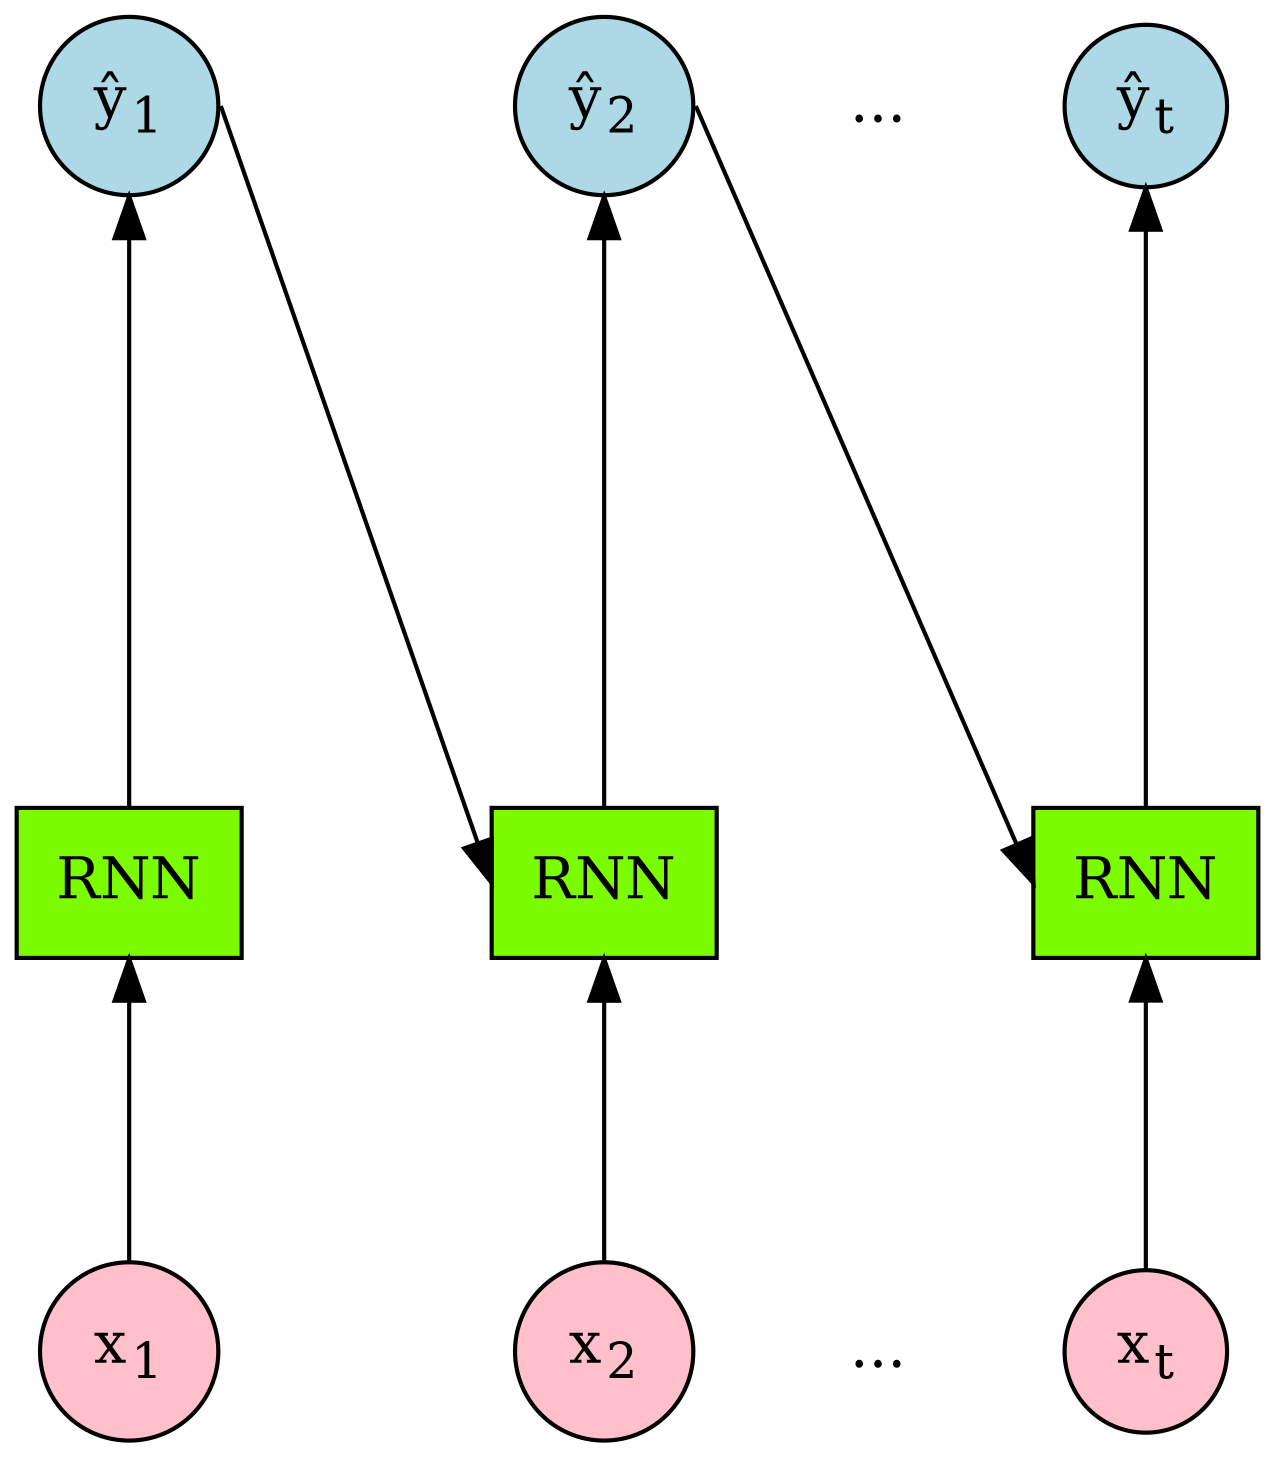
\includegraphics[height=6cm, width=7cm, keepaspectratio]{graphs/recurrent_7.png}
\end{center}}
\end{frame}

\section{LSTM hálózatok}

\begin{frame}
\tableofcontents[currentsection]
\end{frame}

\begin{frame}{Hagyományos RNN hálózat}
A hagyományos LSTM hálózat két bemenete az $x_t$  \textbf{input vektor aktuális eleme} és a $h_{t-1}$ \textbf{előző cella aktiváció}. Ez alapján állítja elő az aktuális cella állapotot:
\begin{columns}
\begin{column}{.5\textwidth}
\begin{block}{}
\vspace{-0.5cm}
\[
h_t = tanh\left(W_h \cdot h_{t-1} + W_x \cdot x_t + b_h\right)
\]
\end{block}
Ennek az architektúrának több hátránya is van:
\begin{itemize}
	\item Igazából \textbf{csak egy nagyon mély hálózat}. 
	\item A hiperbolikus tangens függvény gradiensei \textbf{a szélsőértékek felé haladva eltűnnek}. 
\end{itemize}
\end{column}
\begin{column}{.5\textwidth}
\begin{center}
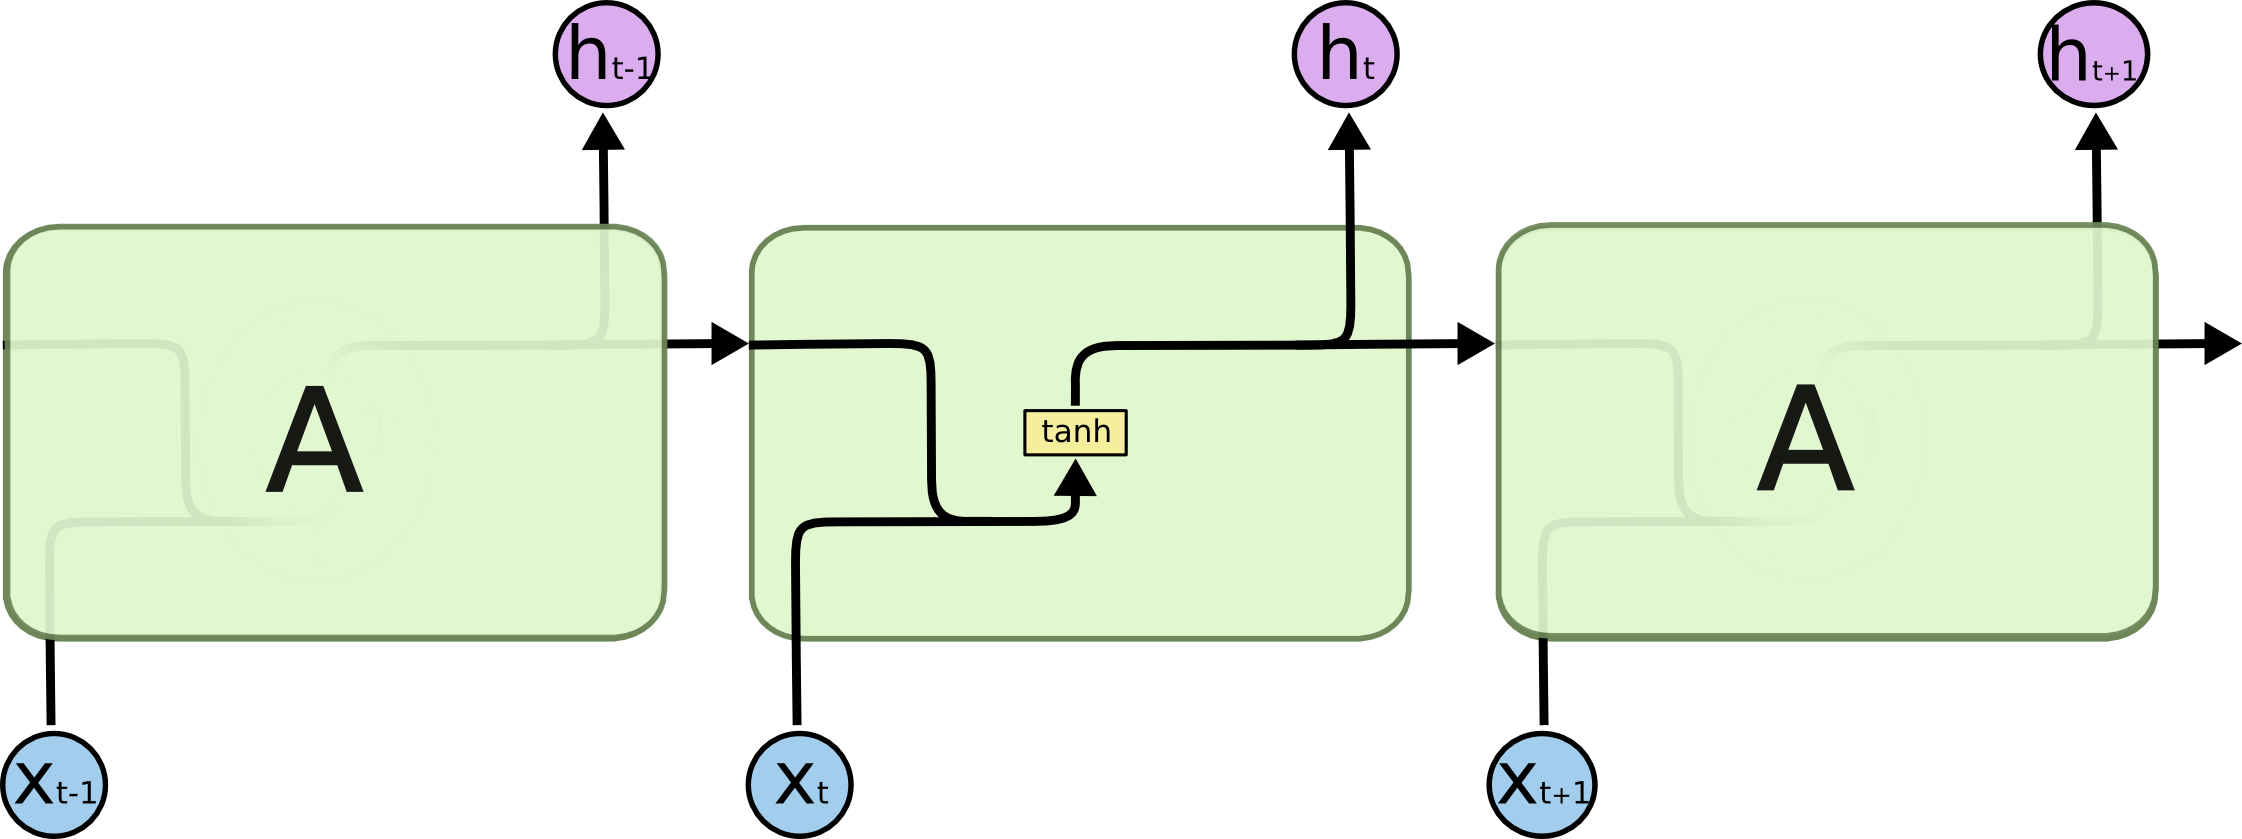
\includegraphics[height=7cm, width=7cm, keepaspectratio]{images/recurrent_5.png}
\end{center}
\end{column}
\end{columns}
\end{frame}

\begin{frame}{LSTM mint az RNN kiterjesztése}
\begin{columns}
\begin{column}{.35\textwidth}
\begin{block}{LSTM architektúra}
Az LSTM (Long Short Term Memory) egy speciális neurális hálózat \textbf{architektúra szekvenciális adatok feldolgozására}.\par\smallskip
\textbf{Memóriacellákból} és különböző \textbf{kapukból} (\textbf{input}, \textbf{felejtés}, \textbf{output}) áll amelyek segítik az információfolyam irányítását.  
\end{block}
\end{column}
\begin{column}{.65\textwidth}
\begin{center}
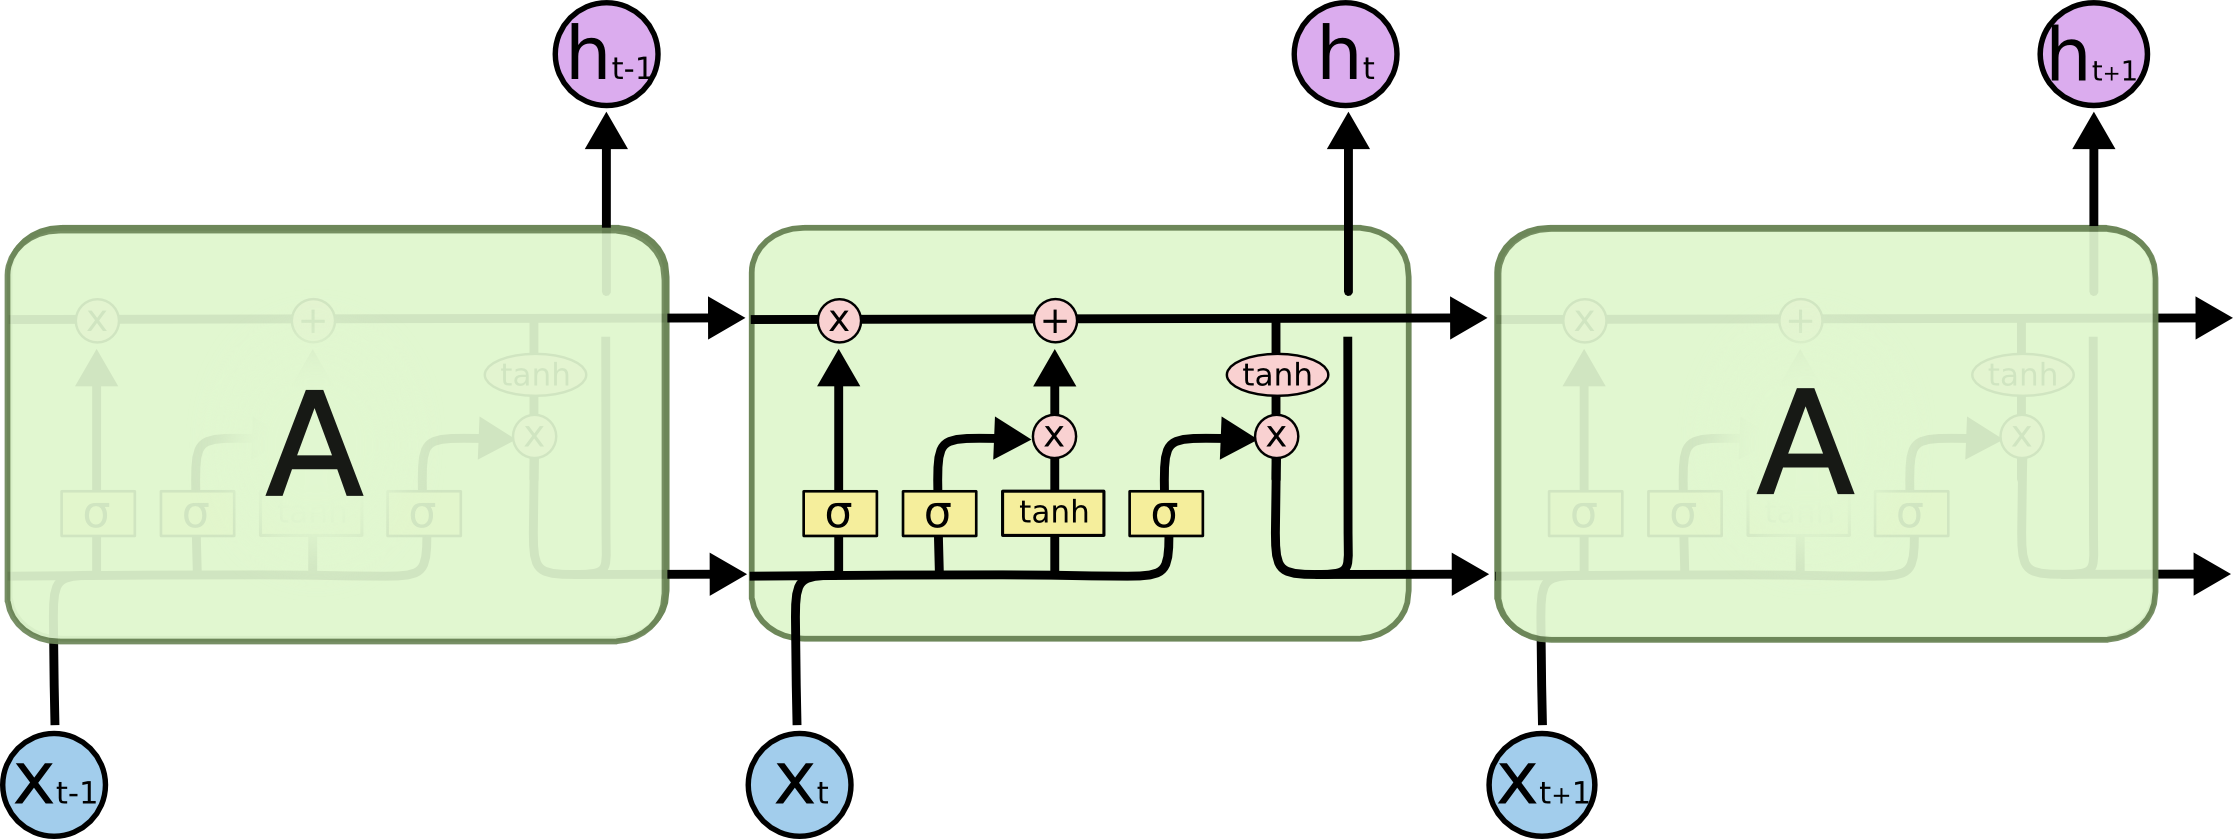
\includegraphics[height=7cm, width=9.5cm, keepaspectratio]{images/recurrent_6.png}
\end{center}
\end{column}
\end{columns}
\end{frame}

\begin{frame}{LSTM cella felépítése}
\begin{columns}
\begin{column}{.4\textwidth}
\only<1>{\begin{block}{Cella állapot}
A cella állapot ($C_t$) LSTM hálózatokban egy \textbf{hosszútávú memória} ami \textbf{több időlépésen keresztül} képes információt eltárolni.\par\smallskip
A cella \textbf{állapot kapukon keresztül képes változni}, amik meghatározzák, hogyan adódik hozzá vagy vonódik ki információ a cella állapotból. 
\end{block}}
\only<2>{\begin{block}{Cella output}
A cella outputja ($h_t$) \textbf{a hálózat aktivációja} $t$ időlépésben.\par\smallskip
A cella outputja az input vektor $t$. eleme és az előző cella aktivációja $h_{t-1}$ alapján áll elő és a következő, $t+1$-edik cella inputjául szolgál. 
\end{block}}
\end{column}
\begin{column}{.6\textwidth}
\begin{center}
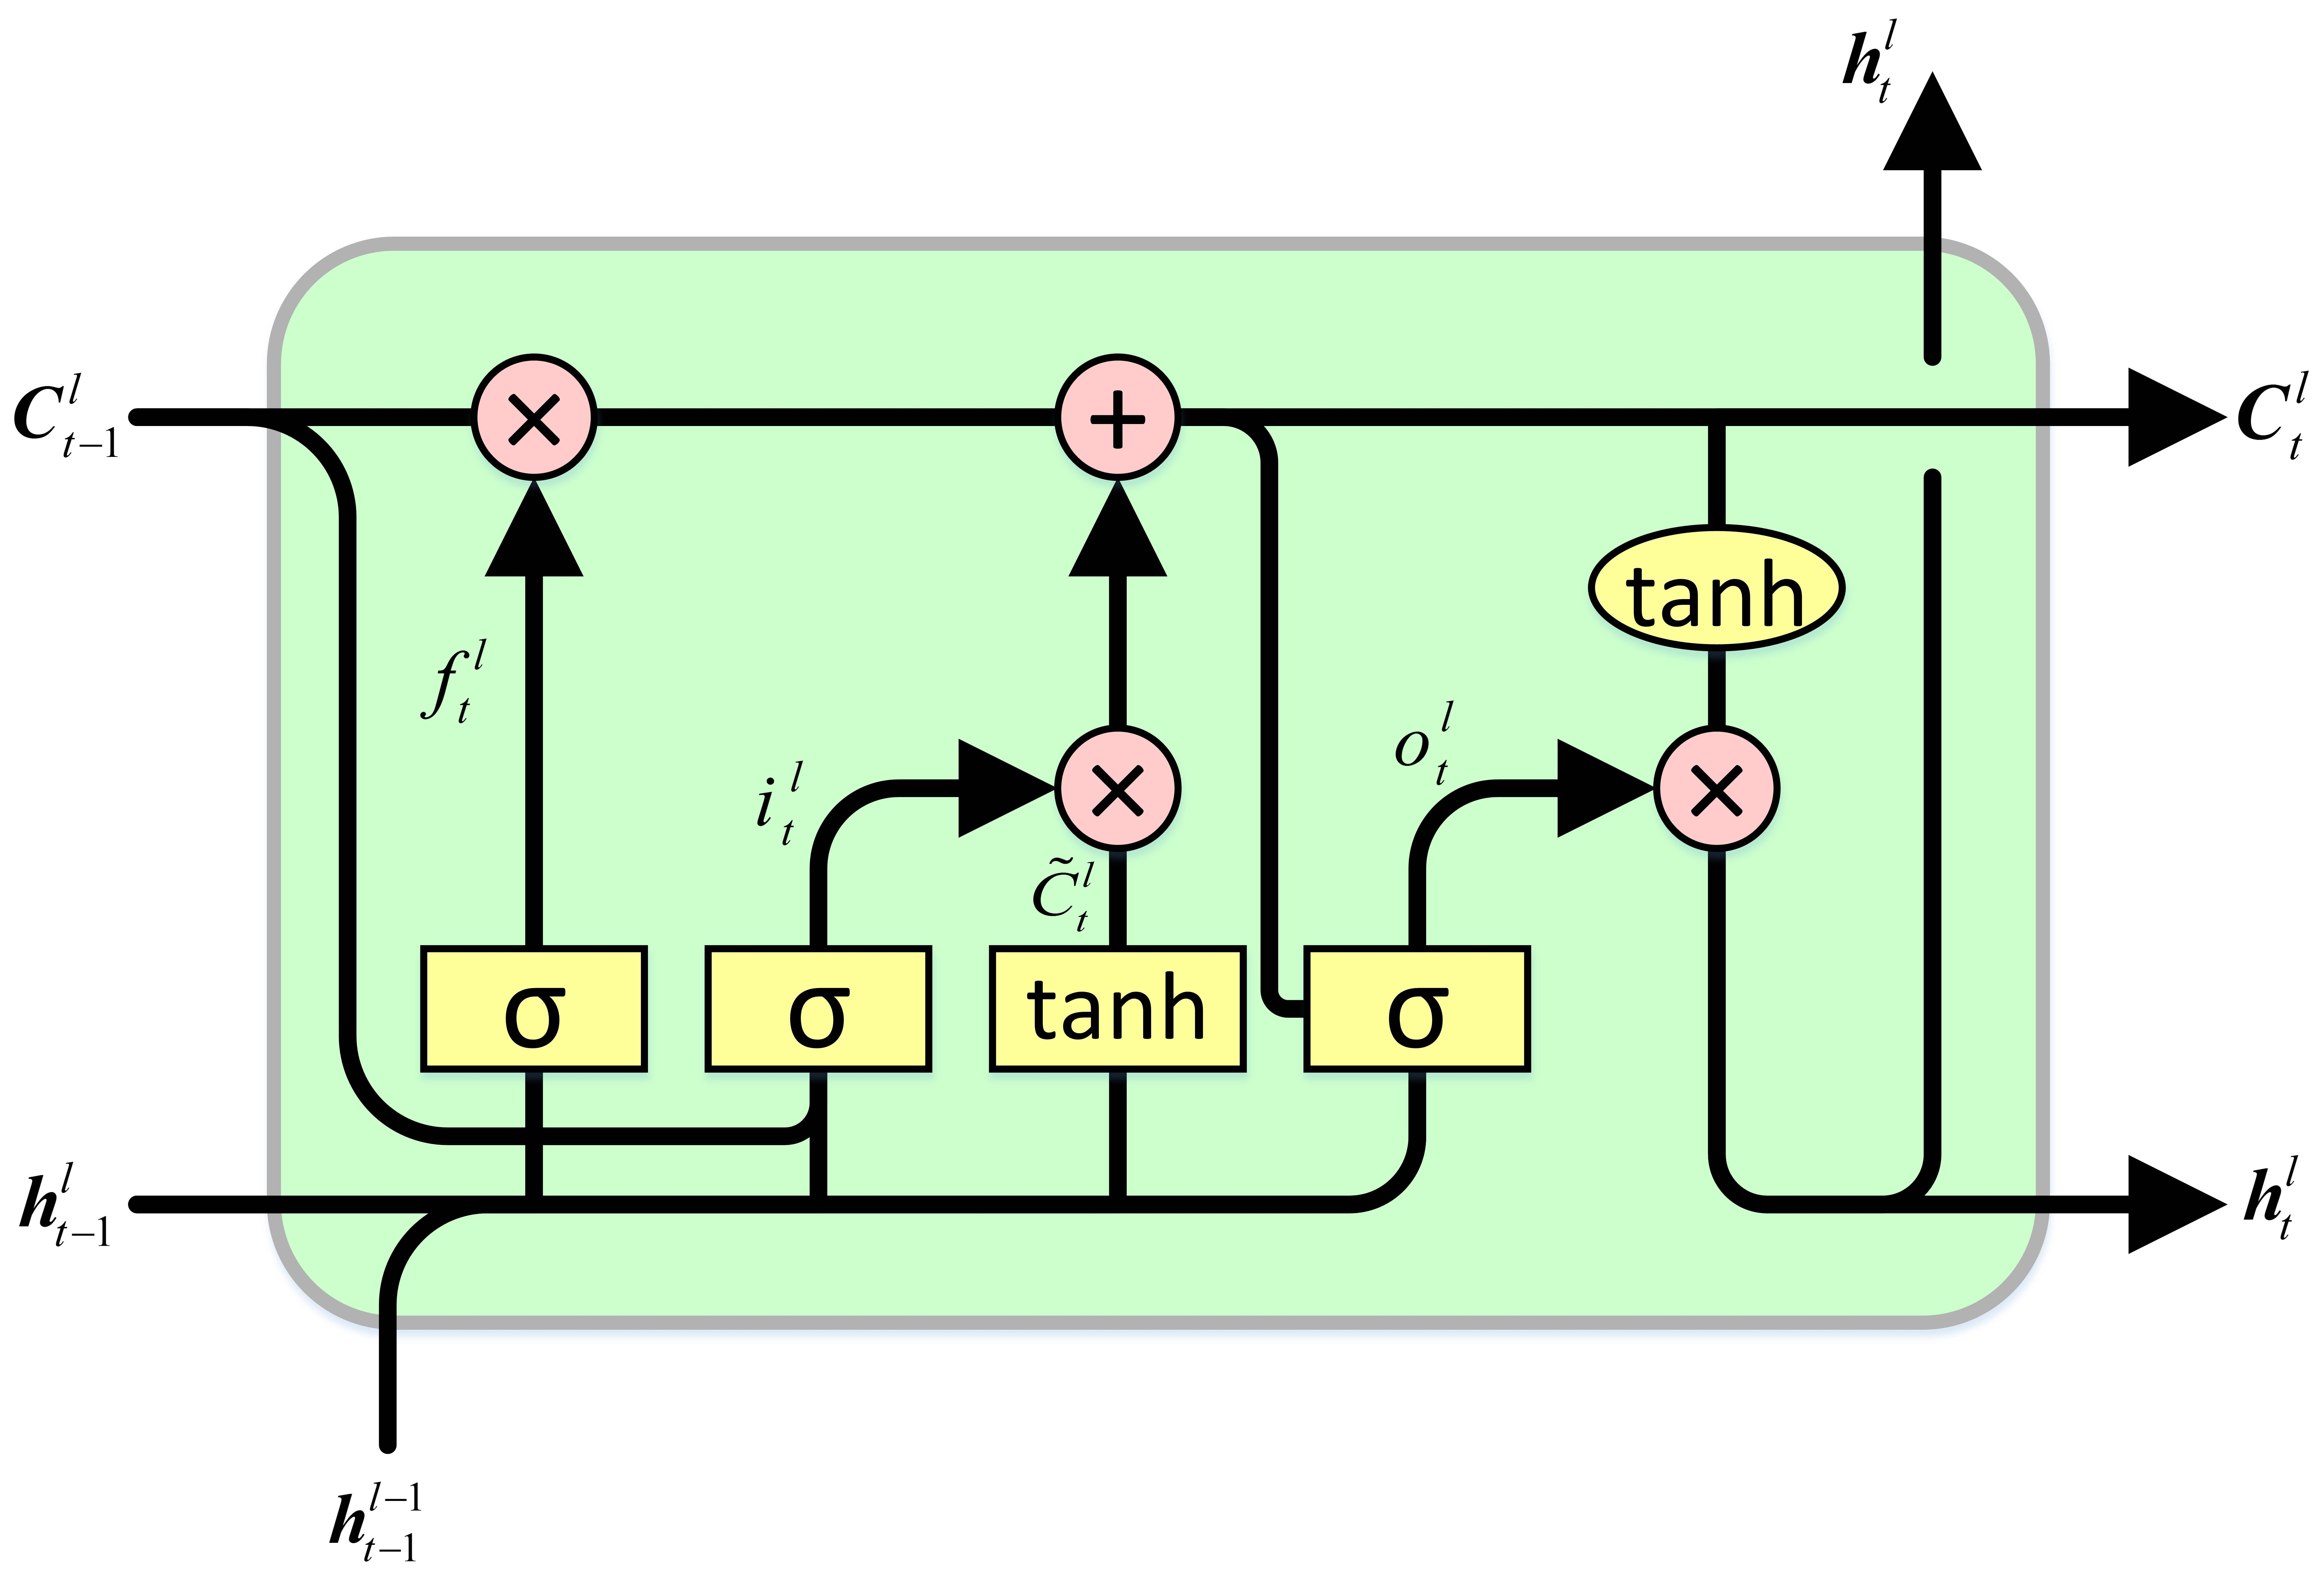
\includegraphics[height=7cm, width=8.5cm, keepaspectratio]{images/recurrent_12.png}
\end{center}
\end{column}
\end{columns}
\end{frame}

\end{document}









